\documentclass[titlepage,openright,letterpaper,12pt]{book}
\usepackage{entete,commandes} % Load les packages et définit des commandes.

%=============================================================================%

% On crée des bools qui sont False par défaut.
\newtoggle{VersionLivre}
\newtoggle{LivrePGChVide}
\newtoggle{ForceEntete}
\newtoggle{AuteureFemme}
\newtoggle{MemoirePasThese}
\newtoggle{useCustomFonts}
\newtoggle{generatePDFa}
\newtoggle{IntroConcluSansNombre}

% Switchboard, l'endroit ou on ajuste les toggles.
% Décommenté -> True; commenté -> False

%\toggletrue{VersionLivre}          % Décommenter pour faire la version livre
%\toggletrue{LivrePGChVide}         % Page gauche de chapiter vide en mode livre.
%\toggletrue{ForceEntete}            % Entête même pour version électronique.
%\toggletrue{AuteureFemme}          % Décommenter si l'auteur est une femme.
\toggletrue{MemoirePasThese}       % Décommenter dans le cas d'un mémoire.
\toggletrue{IntroConcluSansNombre}  % Intro et conclusion non numérotées
\toggletrue{useCustomFonts}         % Fonts différents, voir switchboard.tex.
%\toggletrue{generatePDFa}           % Génère un PDFa plutôt qu'un PDF standard.

%=============================================================================%

\title          {Échantillonage et comptage avec les algorithmes variationnels quantiques} % Pour la page de titre/jury.
% Titre alternatif: Échantillonage et comptage avec les algorithmes variationnels quantiques
\author         {Julien Drapeau}  % Idem
\Organisation   {UNIVERSITÉ de SHERBROOKE}
\Location       {Sherbrooke, Québec, Canada}
\ResumeCourt    {On présente des résultats nouveaux dans un domaine en pleine effervescence.}
\date           {\today}       % Idem
\MotsClefs      {Mots-Clefs \sep Pertinents \sep avec séparateurs}

% On cache le code exécuté dans ce fichier parce qu'il est laid et impertinent.
\begin{comment}
\end{comment}

%=============================================================================%

\makeatletter   % Permet d'accèder aux variables @

%=============================================================================%

    % PDFA-1b/Hyperref
    \iftoggle{generatePDFa}
    {
        % PDF/A stuff (experimental)
        \usepackage[a-1b]{pdfx}
    }
    {
        \newcommand{\sep}{, }
    }
        \usepackage{filecontents}
        \begin{filecontents*}{\jobname.xmpdata}
                \Title          {\@title}
                \Author         {\@author}
                \Subject        {\ResumeCourt}
                \Org            {\Organisation}
                \Keywords       {\MotsClefs}
                \PublicationType{book}
        \end{filecontents*}
        % Couleurs moins intenses, https://ethanschoonover.com/solarized/
        \definecolor{solblue}{HTML}{268bd2}
        \definecolor{solred}{HTML}{dc322f}
        \definecolor{solviolet}{HTML}{6c71c4}
        \definecolor{solmagenta}{HTML}{d33682}
        \definecolor{solcyan}{HTML}{2aa198}
        \definecolor{solorange}{HTML}{cb4b16}
        \definecolor{solyellow}{HTML}{b58900}
        \definecolor{solgreen}{HTML}{859900}
        % Hyperrefs
        \usepackage{hyperref}
        \hypersetup{
            pdfauthor={\@author},
            pdftitle={\@title},
            pdfsubject={\ResumeCourt},
            pdfkeywords={\MotsClefs},
            hyperindex=true,
            bookmarks=true,
            pdfa,
            %pdftex,
            colorlinks=true,
            breaklinks=true,
            urlcolor=mydarkred,
            %linkcolor=solblue!85!black, % A little darker
            linkcolor=mydarkblue,
            citecolor=solcyan,
            bookmarksopen=true,
            unicode=true
        }
        % \usepackage[hyperpageref]{backref}      % Backrefs!
        % \renewcommand{\backref}[1]{[cf.~p.~#1]} % Volé cette ligne à Samuel Boutin
        \usepackage{bookmark}
        \usepackage{cmap} % Doit être après hyperref pour être compatible avec pdf-a

%=============================================================================%

    \iftoggle{useCustomFonts}
    {   
        % Deux prochaines lignes -> Pagella et Mathpazo
        \usepackage{mathpazo} % utilise Palatino pour les mathématiques (mettre en premier)
        \usepackage{tgpagella} % utilise la police TeX Gyre Pagella

        % Deux prochaines lignes -> New Century et Fourier
        %\usepackage{newcent}
        %\usepackage{fouriernc}
        
        \renewcommand{\dagger}{\text{\textdagger}} % Millennial missing dagger fix
        \renewcommand{\iint}{\int\!\!\int}  % Better spacing
        \renewcommand{\iiint}{\int\!\!\int\!\!\int}
        \renewcommand{\iiiint}{\int\!\!\int\!\!\int\!\!\int}
    }
    {}

%=============================================================================%
    
    \iftoggle{AuteureFemme}
    { \newcommand{\monsieurMadame}{Mme.} }    
    { \newcommand{\monsieurMadame}{M.} }

%=============================================================================%

    \iftoggle{MemoirePasThese}
    {   % Si c'est un mémoire
        \newcommand{\documentPresente}{Mémoire présenté}
        \newcommand{\leDocument}{le mémoire}
        \newcommand{\leGrade}{maître ès science (M.Sc.)}
    }
    {   % Si c'est une thèse
        \newcommand{\documentPresente}{Thèse présentée}
        \newcommand{\leDocument}{la thèse}
        \newcommand{\leGrade}{docteur ès science (Ph.D.)}
    }

%=============================================================================%
    
    % Gestion de la version électronmique vs celle imprimée.
    \iftoggle{VersionLivre}
    {   % On fait la version imprimée!

        % On utilise un fontsize plus petit(10pt vs 12pt).
        \let\small\relax
        \let\footnotesize\relax
        \let\scriptsize\relax
        \let\tiny\relax
        \let\large\relax
        \let\Large\relax
        \let\LARGE\relax
        \let\huge\relax
        \let\Huge\relax
        \input{size10.clo}  % Ajuste le fontsize ET les marges
        \geometry{twoside=true, bottom=2.54cm} % L'ordre est important, pour les marges/fontsize.
        %\widowpenalty5000  % Décommenter s'il y a trop de ligne veuves/orphelines.
        %\clubpenalty5000   


        % On enlève la numérotation des pages vides
        \let\origdoublepage\cleardoublepage
        \newcommand{\clearemptydoublepage}{%
            \clearpage%
            {\pagestyle{empty}\origdoublepage}%
            }
        \let\cleardoublepage\clearemptydoublepage
        
        % Permet de mettre un page blanche seulement dans la version imprimée
        \newcommand{\autoPageBlancheLivre}{\clearpage\null\thispagestyle{empty}}

        \iftoggle{LivrePGChVide}
        {
            \let\stdchapter\chapter
            \renewcommand\chapter{\clearpage\null\thispagestyle{empty}\stdchapter}
            \renewcommand{\autoPageBlancheLivre}{}

            \let\stdpart\part
            \renewcommand\part{\clearpage\null\thispagestyle{empty}\stdpart}

            \renewcommand\@endpart{\vfil
                          \if@twoside
                            \null
                            \thispagestyle{empty}%
                            \newpage
                          \fi
                          \if@tempswa
                            \twocolumn
                          \fi}
        }{}

        % Les hyperliens n'ont pas desoins d'être colorés
        \hypersetup{hidelinks}
        % On affiche les DOI dans la biblio -> Pratique en version imprimée
        \bibliographystyle{nature-fr-showdoi}
        % On garde les entêtes dans la bibliographie
        \newcommand{\bibpagestyle}{}
    }
    {   % S'il y a un côté, on fait la version électronique.
        \geometry{letterpaper, lmargin=1.25in, rmargin=1.25in,
                  tmargin=1.5in, bmargin=1.0in, twoside=false}
        \iftoggle{ForceEntete}
        {
            % On garde les entêtes dans la bibliographie
            \newcommand{\bibpagestyle}{}
        }
        {
        % Prochaines lignes enlèvent l'entête
            \renewcommand{\chaptermark}[1]
                {\markboth{{\thechapter. #1}}{}}
            \renewcommand{\sectionmark}[1]{}
            % On enlève les entêtes dans la bibliographie
            \newcommand{\bibpagestyle}{\pagestyle{plain}}
        }

        % On n'affiche pas les DOI dans la biblio -> Plus propre
        % \bibliographystyle{nature-fr}
        %\bibliographystyle{unsrt-fr} % unsrt partiellement traduit. Préférer nature.
        
        % Permet de mettre un page blanche seulement dans la version imprimée
        \newcommand{\autoPageBlancheLivre}{}
    }
    \iftoggle{IntroConcluSansNombre}
    {
        \newcommand{\Introduction}{\chapter*{Introduction}
            \addcontentsline{toc}{chapter}{Introduction}}
        \newcommand{\Conclusion}{\chapter*{Conclusion}
            \addcontentsline{toc}{chapter}{Conclusion}}
    }
    {
        \newcommand{\Introduction}{\chapter{Introduction}}
        \newcommand{\Conclusion}{\chapter{Conclusion}}
    }


%=============================================================================%

\makeatother    % Plus d'accès aux variables @


%=============================================================================%

\begin{document}

%=============================================================================%
% Titre
\begin{comment}
\end{comment}
\makeatletter   % Permet d'accèder aux variables @

\thispagestyle{empty}  % Page blanche avec formattage manuel
\pagenumbering{gobble} % Aucune numérotation, sinon hypperref bug
\vglue 2cm
\begin{center}
    \doublespacing{
    {\LARGE \@title}\\
    \vspace{2.0cm}
    par\\
    \vspace{2.0cm}
    {\large \@author}
    \vspace{2.0cm}\\
    \documentPresente\ au département de physique\\
    en vue de l'obtention du grade de \leGrade
    \vfill
    FACULTÉ des SCIENCES\\
    \Organisation\vspace{1.0cm}\\
    \Location, \@date  % La date sera celle de la compilation
    }
\end{center}

\makeatother    % Plus d'accès aux variables @


\frontmatter % Pagination de préambule

% Jury
\begin{comment}
\end{comment}
\makeatletter   % Permet d'accèder aux variables @

\iftoggle{LivrePGChVide}
{}
{
    % Next two lines force a linebreak in ebook versions
    \chapter*{}
    \vspace{-4.7cm}
}

\thispagestyle{empty}

\begin{center}
    \vglue 2cm
    Le 10 mai 2025 \\ 
    %Le \@date % Lorsque le document sera accepté!
    \vspace{2cm}
    \scalebox{1} % Empêche le retour à la ligne si le nom est trop long.
    {\it le jury a accepté \leDocument\ de \monsieurMadame~\@author~dans sa version finale.} 
    
    \vspace{2cm}
    Membres du jury\\
    \vspace{2cm}

    Professeur Stefanos Kourtis\\
    Directeur de recherche\\
    Département de physique\\
    \vspace{2cm}
    
    Professeur André-Marie Tremblay\\
    Membre interne\\
    Département de physique\\
    \vspace{2cm}

    Professeur Baptiste Royer\\
    Président rapporteur\\
    Département de physique\\
    \vspace{2cm}
\end{center}

%\clearpage

\makeatother    % Plus d'accès aux variables @


% Dédicace
\begin{comment}
\end{comment}

\chapter*{}
\vspace{-10pt}
\setlength\epigraphwidth{.5\textwidth}
\setlength\epigraphrule{0\textwidth}
\epigraph{« Je vis parce que les montagnes ne savent pas rire, ni les vers de terre chanter. »}{- Emil Cioran}
\thispagestyle{empty}

% Sommaire
\clearpage % Mets le sommaire à la bonne page dans la TOC
\chapter*{Sommaire}
\addcontentsline{toc}{chapter}{Sommaire}
En exploitant à la fois les ressources classiques et quantiques, les algorithmes variationnels quantiques peuvent exécuter des tâches computationnelles complexes sur des ordinateurs quantiques bruités, sans nécessiter de correction d'erreurs. Ces algorithmes visent notamment à résoudre des problèmes d'optimisation combinatoire, se plaçant ainsi en concurrence avec des algorithmes classiques perfectionnés au fil des décennies. Une approche complémentaire consiste à se tourner vers des problèmes intrinsèquement plus complexes: les problèmes de dénombrement. Ces derniers, qui consistent à compter le nombre de solutions aux problèmes de décision, pourraient se révéler plus accessibles aux algorithmes variationnels quantiques qu'aux algorithmes classiques.

Dans le cadre de ce mémoire, un algorithme surnommé VQCount est introduit pour la résolution de problèmes de dénombrement. VQCount s'appuie sur l'équivalence entre l'échantillonnage aléatoire et le comptage approximatif pour estimer le nombre de solutions à un facteur multiplicatif près, en exploitant l'ansatz quantique à opérateurs alternants comme générateur de solutions. Cette approche nécessite l'échantillonnage d'un nombre polynomial de solutions selon la taille du problème, même lorsque ce dernier possède un nombre exponentiel de solutions, ce qui constitue une amélioration exponentielle par rapport à des travaux précédents.

À l'aide de simulations de réseaux de tenseurs, la performance de VQCount avec des circuits de faible profondeur est étudiée sur des instances synthétiques de deux problèmes \textsf{\#P}-difficile, positif \#1-in-3SAT et positif \#NAE3SAT, en employant comme générateurs de solutions l'algorithme quantique d'optimisation approximative ainsi que l'ansatz quantique à opérateurs alternants avec forçage de Grover. Un compromis entre la probabilité de succès et l'uniformité de l'échantillonnage du générateur est observé et exploité pour atteindre un gain en efficacité exponentiel par rapport à l'échantillonnage par rejet naïf. Ces résultats soulignent le potentiel et les limites des algorithmes variationnels quantiques pour le comptage approximatif.

\noindent
\textbf{Mots-clés:} Algorithmes variationnels quantiques, Échantillonnage aléatoire, Comptage approximatif, Auto-réductibilité, Satisfaisabilité, Réseaux de tenseurs

% Remerciements
\chapter*{Remerciements}
\begin{comment}
\end{comment}

% Ma mère et mes soeurs,

% Justin, Léanne, Thibault, Thomas, Philippe et William,

% Sovannie,

% Antoine, Benjamin, Jérémie, Martin, Pierre-Alexandre et tous les membres du groupe,

% Stefanos,



% Tables des matières/Figures
{
    \setlength{\parskip}{0ex}
    \tableofcontents
    \listoffigures
    %\listoftables
}

%=============================================================================%

\mainmatter % Pagination standard
\onehalfspacing

%-----------------------------------------------------------------------------%

% \include serait préférable à \input à partir d'ici, mais MiKTeX sur Windows
% n'aime pas les \cite dans un \include. Fonctionne parfaitement sur TeXLive.

\Introduction   % Chapitre qui ne sera pas numéroté si IntroConcluSansNombre est Vrai

%-----------------------------------------------------------------------------%

En exploitant les principes du parallélisme, de la superposition et de l'intrication, les algorithmes quantiques remettent en question les limites classiques du calcul, promettant des accélérations exponentielles pour certains types de problèmes. L'algorithme de Shor, par exemple, permet de factoriser des entiers naturels en offrant une accélération superpolynomiale par rapport aux 
meilleurs algorithmes classiques connus~\cite{shorAlgorithmsQuantumComputation1994}. Bien que le calcul quantique soit prometteur, son utilité pratique reste floue pour diverses raisons. Les algorithmes quantiques ne s'appliquent en ce moment qu'à une classe de problèmes restreints, et leurs applications restent limitées. En outre, les ordinateurs quantiques actuels, appelés ordinateurs quantiques à échelle intermédiaire bruités, sont affligés par différentes complications rendant tout calcul excessivement difficile: un nombre restreint de qubits, une connectivité limitée et la présence d'erreurs entravant la taille des circuits.

Pour contourner ces difficultés, les algorithmes variationnels quantiques (VQA) furent conçus pour exploiter les mécanismes du calcul quantique, tout en tirant profit de la puissance du calcul classique~\cite{cerezoVariationalQuantumAlgorithms2021}. Ces algorithmes visent à résoudre des problèmes complexes en utilisant l'état préparé par un circuit quantique paramétré, dont les paramètres sont ajustés par un optimiseur classique pour minimiser la fonction de coût du problème. Étant basée sur l'optimisation de paramètres, cette stratégie permet de considérer toutes les difficultés précédentes d'un seul coup, tout en limitant la taille des circuits quantiques. Au cours des dernières années, de nombreux travaux ont tenté de perfectionner les VQA en développant par exemple des techniques permettant une meilleure exploitation de la structure des problèmes. Toutefois, il reste encore à déterminer si ces algorithmes présentent un réel avantage par rapport aux algorithmes classiques.  

Les VQA sont principalement utilisés pour résoudre des problèmes d'optimisation combinatoire, tels que le problème de coupe maximale et le problème des ensembles indépendants. Comme des solveurs classiques pour ce type de problème ont été développés au fil des décennies, il est difficile de démontrer la supériorité des VQA. Le projet de ce mémoire propose une approche différente pour aborder cette question. Plutôt que de rivaliser avec des algorithmes classiques hautement performants, les VQA sont appliqués à la résolution de problèmes vastement plus complexes: les problèmes de dénombrement, ou plus simplement les problèmes de comptage. Ceux-ci sont difficiles même pour les algorithmes classiques, mais potentiellement moins pour les algorithmes quantiques. Au lieu de chercher une solution quasi optimale, les problèmes de dénombrement s'intéressent plutôt à déterminer le nombre de solutions respectant les contraintes du problème. Les problèmes de comptage, qui font partie de la classe de complexité \textsf{\#P}, se situent au-dessus des problèmes d'optimisation typiques dans la hiérarchie de la complexité computationnelle.

Pour répondre à cette question, l'équivalence entre le comptage approximatif et l'échantillonnage quasi uniforme, établie par Jerrum, Valiant et Vazirani~\cite{jerrumRandomGenerationCombinatorial1986}, est utilisée. Cette correspondance donne lieu à un algorithme randomisé de comptage approximatif, surnommé algorithme de JVV, permettant l'estimation à un facteur multiplicatif près du nombre de solutions à un problème de comptage auto-réductible si les solutions peuvent être échantillonnées suffisamment uniformément. Cet algorithme exploite la propriété d'auto-réductibilité de certains problèmes, c'est-à-dire la capacité à utiliser la structure inhérente au problème pour sa résolution.

L'algorithme VQCount, introduit dans ce mémoire, fait le pont entre les VQA et les problèmes de comptage. Cet algorithme montre qu'il est possible d'utiliser les VQA pour construire un solveur approximatif aux problèmes \textsf{\#P}. Pour ce faire, VQCount prépare une distribution d'états contenant une superposition de solutions au problème de comptage avec une haute probabilité en utilisant un VQA nommé ansatz quantique à opérateurs alternants (QAOA)~\cite{hadfieldQuantumApproximateOptimization2019}. Après avoir modifié le circuit quantique de QAOA pour tirer avantage de la propriété d'auto-réductibilité, VQCount emploie l'algorithme de comptage approximatif pour estimer le nombre de solutions à partir de la distribution préparée. Si QAOA échantillonne des solutions suffisamment près de l'uniformité avec un taux de succès fini, alors seulement un nombre polynomial d'échantillons est nécessaire pour estimer le nombre de solutions avec l'algorithme de JVV. 

Grâce aux simulations de réseaux de tenseurs, cette étude évalue la performance de VQCount sur des circuits quantiques de faible profondeur appliqués à des instances synthétiques de deux problèmes \textsf{\#P}-difficile: positif \#1-in-3SAT et positif \#NAE3SAT. Les solutions sont générées à l'aide de l'algorithme quantique d'optimisation approximative (QAOA)~\cite{farhiQuantumApproximateOptimization2014} et de l'ansatz quantique à opérateurs alternants avec forçage de Grover (GM-QAOA)~\cite{bartschiGroverMixersQAOA2020}. Cette analyse met en évidence un équilibre entre la probabilité de succès et l'uniformité de l'échantillonnage, qui permet d'obtenir un gain exponentiel en efficacité par rapport à une approche naïve par rejet. Ces résultats révèlent à la fois les atouts et les limites des algorithmes variationnels quantiques pour le comptage approximatif.

Le chapitre~\ref{cha:complexite-du-denombrement} explore en détail les problèmes de dénombrement avec le langage de la théorie de la complexité. L'algorithme de JVV et ses concepts sous-jacents, c'est-à-dire l'auto-réductibilité, l'échantillonnage aléatoire et le comptage approximatif, sont présentés au chapitre~\ref{cha:echantillonnage-quasi-uniforme-comptage-approximatif-randomise}. Les algorithmes variationnels quantiques sont présentés de manière générale au chapitre~\ref{cha:algorithmes-variationnels-quantiques} avec un accent sur QAOA et GM-QAOA. L'algorithme VQCount, fruit de ce travail, est détaillé au chapitre~\ref{cha:comptage-variationnel-quantique}. La performance de VQCount est finalement caractérisée au chapitre~\ref{cha:resolution-de-problemes-avec-vqcount}. L'annexe~\ref{ann:expression-fermee-etat-circuit-gm-qaoa} dérive une expression fermée de l'état préparé par un circuit GM-QAOA, alors que l'annexe~\ref{ann:simulation-circuits-quantiques-avec-reseaux-de-tenseurs} introduit les méthodes de réseaux de tenseurs utilisées pour la simulation de circuit quantique de l'algorithme VQCount.

Le travail effectué au cours de ce projet a mené à la publication d'un manuscrit sur arXiv: \url{https://arxiv.org/abs/2503.07720}. Ce mémoire prend ainsi son inspiration de cet écrit.

\begin{comment}
Problème NP vs #P
Théorème de Toda
Description du paper JVV
Complexité exacte vs approximative
Countage exact vs approximatif
Borne sur le comptage ("a tighter bound for counting max-weight solutions to 2SAT instances" ou l'équivalent pour 3SAT)
\end{comment}

\chapter{Complexité du dénombrement}
\label{cha:complexite-du-dénombrement}

\begin{comment}
    \subsection*{Plan}
    
    \begin{enumerate}
        \item Introduire les problèmes algorithmiques difficiles
        \item Décrire les applications de ces problèmes
        \item Expliquer les prochaines sections
        \item Expliquer pourquoi on ne parle pas des machines de Turing (thèse de Church-Turing)
    \end{enumerate}
\end{comment}

Qu'est-ce qu'un problème de dénombrement? Simplement, un tel problème consiste à déterminer le nombre de solutions respectant un ensemble de contraintes. Les problèmes de dénombrement, ou de comptage, font partie des problèmes computationnels difficiles, ce qui signifie qu'il est peu probable que ces problèmes soient résolubles efficacement. Les problèmes de comptage surgissent dans de nombreuses disciplines, avec des applications en raisonnement probabiliste~\cite{rothHardnessApproximateReasoning1996, sangPerformingBayesianInference2005, abramsonHailfinderBayesianSystem1996}, en fiabilité des réseaux~\cite{valiantComplexityEnumerationReliability1979, duenas-osorioCountingbasedReliabilityEstimation2017}, en mécanique statistique~\cite{jerrumPolynomialTimeApproximationAlgorithms1993} et en intelligence artificielle~\cite{balutaQuantitativeVerificationNeural2019}. Contrairement à certains problèmes étudiés dans le domaine du calcul quantique, comme l'échantillonnage de bosons~\cite{aaronsonComputationalComplexityLinear2011} ou l'échantillonnage de circuits aléatoires~\cite{boulandComplexityVerificationQuantum2019}, une solution à ces problèmes peut avoir un impact concret, justifiant alors l'étude de tels problèmes.

Ce chapitre décrit le cadre théorique entourant la classe des problèmes de dénombrement en détail. Pour ce faire, celle-ci est définie à l'aide du langage de la théorie de la complexité à la section~\ref{sec:classes-de-complexite}. Le problème de comptage prototypique, le problème de satisfaisabilité, sert d'exemple et est décrit à la section~\ref{sec:satisfaisabilite-booleenne}. Celui-ci est d'une grande importance pour ce projet et est ainsi référencé tout au long de ce mémoire. La section~\ref{sec:intractabilite-approximation-et-optimisation} explique l'importance des méthodes approximatives alors que la section~\ref{sec:comptage-de-modeles} décrit les solveurs modernes pour les problèmes de comptage. Finalement, le comportement des instances aléatoires pour ces problèmes est présenté à la section~\ref{sec:transitions-de-phase}, où des transitions de phase font étonnamment leurs apparitions.

Il est souvent favorable de décrire la théorie de la complexité à l'aide du concept de \textit{machine de Turing}. Cependant, ce mémoire suppose que la thèse de Church-Turing soit vraie, et donc que n'importe quel modèle de calcul puisse être utilisé de manière équivalente, pour faire abstraction de ce langage et simplifier les idées présentées.

%-----------------------------------------------------------------------------%

\section{Classes de complexité}
\label{sec:classes-de-complexite}

\begin{comment}
\subsection*{Plan}

\begin{enumerate}
    \item Définir comment quantifier la complexité d'un problème (temps contre espace)
    \item Décrire le but des classes de complexité
    \item Expliquer les propriétés des classes de complexité et leurs relations
    \item Expliquer la notation de la complexité (O notation) et les machines de Turing
    \item Décrire la tour de complexité (hiérarchie polynomiale) 
    \item Comparer les classes importantes: P et NP et \#P
    \item Établir la conjecture P != NP
    \item Mentionner le théorème de Toda
    \item Parler des classes de complexités quantique
    \item Parler de la these de church-turing pour les ordis quantiques
\end{enumerate}

\subsection*{Références}

1. Moore, Cristopher, and Stephan Mertens, The Nature of Computation (Oxford, 2011; online edn, Oxford Academic, 17 Dec. 2013), https://doi.org/10.1093/acprof:oso/9780199233212.001.0001, accessed 19 July 2024.

2. Arora, S. and Barak, B. Computational Complexity: A Modern Approach. (Cambridge University Press, Cambridge, 2009). doi:10.1017/CBO9780511804090.
\end{comment}

La théorie de la complexité s'intéresse à la classification des problèmes algorithmiques en \textit{classes de complexité}, c'est-à-dire en ensembles de problèmes de même complexité. Classifier un problème permet de caractériser les ressources nécessaires pour sa résolution par un algorithme. Les problèmes d'une même classe ont une difficulté intrinsèque similaire, ce qui facilite le choix d'un algorithme et de ressources appropriées. Savoir qu'un problème n'est pas réalistement résoluble, ou plus précisément intraitable, limite les attentes. Sachant ceci, la recherche dans cette direction s'avère grandement utile. La théorie de la complexité cherche aussi à comparer les problèmes de différentes complexités pour comprendre l'espace des problèmes en plus grande profondeur. Comparer des problèmes faciles avec des problèmes difficiles peut par exemple aider à comprendre ce qui rend un problème difficile et donc à trouver des algorithmes résolvant efficacement les problèmes plus complexes. Des liens, nommés réductions, sont définis entre différents problèmes pour comparer leurs complexités. Un algorithme efficace pour un problème peut en effet être efficace pour un différent problème s'il existe une réduction entre ceux-ci. Les classes de complexité, de manière similaire au modèle de la machine de Turing, tentent de définir de manière abstraite la difficulté d'un problème. Quel que soit le matériel informatique à notre disposition, un problème d'une classe donnée ne doit pas changer de classe; un problème simple doit rester simple dans tous les cas.

Comment est-il possible de déterminer la complexité d'un problème? Pour ce faire, les classes de complexité se basent sur les ressources indispensables à la résolution du problème: le temps et la mémoire. Afin de trouver la solution à un problème, un programme doit effectuer un certain nombre d'opérations, limité dans le temps par le matériel informatique. On parle alors de \textit{complexité en temps}. Afin de produire un résultat final, le programme doit garder en mémoire les résultats intermédiaires. Ceux-ci doivent être sauvegardés dans le matériel informatique afin d'être réutilisés ultérieurement. Comme la quantité d'information conservée est aussi un facteur limitant pour le matériel informatique, on parle donc de \textit{complexité en espace}. 

La complexité en temps et en espace d'un problème est définie selon la taille de celui-ci. Afin de capturer cette dépendance, une loi d'échelle est utilisée pour encapsuler la difficulté d'un problème en fonction de sa taille. Le temps et la mémoire quantifient bien les ressources nécessaires des algorithmes. Par contre, ceux-ci dépendent du matériel informatique utilisé. Il est attendu qu'un ordinateur moderne soit bien plus performant qu'une des premières machines analogues. Comment retirer cette dépendance de la notion de complexité? Pour ce faire, on fait appel à la notation asymptotique, communément appelée la \textit{notation $\mathcal{O}$}. La notation asymptotique caractérise la vitesse de croissance d'une fonction en ne considérant que son comportement global à l'infini. Les coefficients ainsi que les termes asymptotiquement inférieurs ne sont pas considérés. Par exemple, pour un problème de taille $n$, la résolution de celui-ci pourrait demander un temps exponentiel $\mathcal{O}(2^{n})$ et une mémoire polynomiale $\mathcal{O}(n)$. Remarquons qu'il n'y a aucune dépendance au matériel informatique: deux ordinateurs différents doivent effectuer le même nombre d'opérations et sauvegarder la même quantité d'information. Un de ces ordinateurs pourrait toutefois résoudre le problème plus rapidement si celui-ci peut effectuer un plus grand nombre d'opérations par seconde ou accéder plus rapidement à sa mémoire. L'attrait des classes de complexité vient donc en partie de cette abstraction du matériel informatique.

La quantification de ces ressources permet la séparation de plusieurs problèmes: il est en effet souhaitable de séparer les algorithmes efficaces de ceux qui ne le sont pas. Commençons par définir deux classes de complexité particulièrement importantes: \textsf{P} et \textsf{NP}. Pour ce faire, un certain type de problème doit d'abord être défini. Un \textit{problème de décision} regroupe simplement tous les problèmes pouvant se répondre par oui ou non. Tout problème de décision $A$ peut être représenté par une fonction $A(x) \in \set{ 0, 1 }$, où $x$ représente une instance du problème. Les problèmes de décision se manifestent fréquemment, tant en informatique qu'en physique. Ceux-ci se présentent sous diverses formes: est-ce qu'un nombre $x$ est premier? La configuration $x$ représente-t-elle un état fondamental du système donné? Est-ce qu'il existe un chemin $x$ parcourant une seule fois toutes les villes d'une région en parcourant au maximum une distance $d$?

Quand peut-on dire qu'un problème de décision est résoluble efficacement? La classe de complexité \textsf{P}, pour « temps polynomial », tente de répondre à cette question. Informellement, un problème de la classe \textsf{P} est un problème de décision qui peut être résolu en temps polynomial. Un problème est donc considéré comme efficacement résoluble ou \textit{traitable}, s'il appartient à la classe \textsf{P}. 

\begin{maindefinition}{Classe de complexité \textsf{P}}{classe-p}
    Une fonction $A$ fait partie de la classe de complexité \textsf{P} si et seulement si elle prend la forme 
    \begin{equation*}
        A(x)=\exists y
    \end{equation*}
    et elle est calculable en temps polynomial, c’est-à-dire en temps $O(n^{c})$ pour une taille $n = \lvert x \rvert$ et une constante $c$, où $\lvert y \rvert = \mathrm{poly}(\lvert x \rvert )$.
\end{maindefinition}

Soit, par exemple, le problème de décision du test de primalité $A$. Ce problème cherche à déterminer si un entier naturel $x$ est premier ou composé. Ce problème peut être résolu, c'est-à-dire qu'il est possible de calculer $A(x)=\exists y$, en temps polynomial $\tilde{O}(\log(n)^{12})$~\cite{agrawalPRIMES2004}, où la notation $\tilde{O}$ signifie que les termes polylogarithmiques sont aussi cachés. 

La relation entre un calcul en temps polynomial et un calcul efficace semble évidente de prime abord. La thèse de Cobham–Edmonds indique en effet qu'un problème algorithmique peut être résolu efficacement s'il est résoluble en temps polynomial~\cite{cobhamIntrinsicComputationalDifficulty1965, edmondsPathsTreesFlowers1965}. Cependant, certains problèmes ne possèdent pas de solutions trouvables efficacement en pratique. Par exemple, un problème peut appartenir à la classe \textsf{P}, mais être doté d'un grand coefficient limitant le calcul. Cela n'étant pas le cas pour la majorité des problèmes, cette supposition s'avère malgré tout une bonne règle empirique. 

Une deuxième classe particulièrement importante en théorie de la complexité est la classe \textsf{NP}, pour « temps polynomial non déterministe ». Celle-ci regroupe les problèmes de décision dont les solutions sont vérifiables en temps polynomial. Généralement, ces problèmes sont formulés sous la forme suivante: existe-t-il une solution, vérifiable en temps polynomial, au problème donné? Malgré que les solutions soient vérifiables efficacement, déterminer l'existence d'une telle solution n'est pas nécessairement possible en temps polynomial. Une métaphore souvent utilisée pour la description d'un problème \textsf{NP} est celle d'une aiguille dans une botte de foin. Trouver cette aiguille parmi la quantité énorme de brins de foin est un défi de taille. Par contre, une fois l'aiguille trouvée, il n'y a aucun doute qu'il s'agit bien d'une aiguille. 

\begin{maindefinition}{Classe de complexité \textsf{NP}}{classe-np}
    Une fonction $A$ fait partie de la classe de complexité \textsf{NP} si et seulement si elle prend la forme
    \begin{equation*}
        A(x) = \exists y \mid B(x,y)
    \end{equation*}
    pour une fonction $B \in  \textsf{P}$, où $\lvert y \rvert = \mathrm{poly}(\lvert x \rvert)$.
\end{maindefinition}

On appelle $B$ le vérificateur du problème de décision $A$ et $y$ le certificat ou le témoin pour l'entrée $x$. Un exemple de problème \textsf{NP} est le problème du commis voyageur. Soit un graphe $x$ représentant les villes d'une région particulière. Est-ce que le commis voyageur peut visiter toutes les villes exactement une fois et revenir à son point de départ en parcourant une distance inférieure à $d$? Dans ce cas, la fonction $A$ détermine le chemin parcouru alors que la fonction $B$ détermine si un chemin $y$ est de taille inférieure à $d$.

La classe \textsf{NP} est aussi définie comme la classe de problèmes pouvant être résolu par une machine de Turing non déterministe en temps polynomiale, d'où son nom. Cette définition est toutefois équivalente à la définition précédente, c'est-à-dire la classe de problèmes vérifiable par une machine de Turing déterministe en temps polynomial~\cite{sipserIntroductionTheoryComputation1996}. Notons que la classe \textsf{P} est contenue dans la classe \textsf{NP}. En effet, comme un problème de \textsf{P} est résoluble en temps polynomial, alors nécessairement une solution à ce problème peut aussi être vérifiée en temps polynomial. Cependant, une question, faisant partie des problèmes du prix du millénaire~\cite{carlsonMillenniumPrizeProblems2006}, demeure ouverte: est-ce que $\textsf{P} = \textsf{NP}$? La conjecture largement répandue répond à cette question par la négative. L'hypothèse de temps exponentiel~\cite{impagliazzoComplexityKSAT2001} suggère par exemple que certains problèmes de \textsf{NP} sont résolubles en temps exponentiel, un résultat significatif sur la difficulté de ces problèmes. En conséquence, un problème est \textit{intraitable} s'il n'est pas résoluble en temps polynomial, par opposition à un problème traitable. 

% \textcolor{mydarkred}{\textit{Conséquences?}}

% \textcolor{mydarkred}{\textit{Parler de non-déterministique. Est-ce pertinent comme il faut introduire les machines de Turing non-déterministe? Autrement, un problème appartient à la classe \textsf{NP} s'il est résoluble en temps polynomial par une machine de Turing non-déterministe. }}

% \textcolor{mydarkred}{\textit{On a donc que $P \subseteq NP$.}}
% \textcolor{mydarkred}{\textit{NP pour temps non-déterministique.}}
% \textcolor{mydarkred}{\textit{La conjecture "Exponential Time Hypothesis" suggère que certains problèmes dans NP prennent un temps exponentiel.  (voir https://arxiv.org/pdf/1611.04471 pour plus d'information)}}

La classe de complexité d'intérêt dans le cadre de ce mémoire est la classe \textsf{\#P} introduit par Valiant~\cite{valiantComplexityComputingPermanent1979}. Cette classe, définie par extension à la classe \textsf{NP}, cherche non seulement à déterminer si un problème de décision possède une solution, mais aussi à spécifier le nombre de solutions à ce problème. Ainsi, un \textit{problème de dénombrement} ou un \textit{problème de comptage} consiste à trouver le nombre de solutions d'un problème de décision. Un problème de comptage est donc défini par rapport à un problème de décision. Prenons par exemple le problème du commis voyageur. Le problème de décision généralement défini cherche un trajet de taille inférieure à une certaine distance. Le problème de comptage adjoint exige alors le nombre de trajets possibles de taille inférieure à la distance donnée. 

\begin{maindefinition}{Classe de complexité \textsf{\#P}}{classe-sharp-p}
    Une fonction $A$ fait partie de la classe de complexité $\textsf{\#P}$ si et seulement si elle prend la forme
    \begin{equation*}
        A(x) = \lvert \set{ y \mid B(x, y)} \rvert
    \end{equation*}
    pour une fonction $B \in \textsf{P}$, où $\lvert y \rvert = \mathrm{poly}(\lvert x \rvert)$ pour toutes les valeurs $y$ prises par $B(x,y)$.
\end{maindefinition}

% \textcolor{mydarkred}{\textit{Changer!}}

Par définition, un problème de la classe \textsf{\#P} est au moins aussi difficile qu'un problème de la classe \textsf{NP}. Connaître le nombre de solutions à un problème de décision indique effectivement s'il existe au moins une solution à un problème de décision. Cependant, les problèmes de comptage intéressants possèdent fréquemment un nombre exponentiel de solutions, impliquant une plus grande complexité inhérente.

% \textcolor{mydarkred}{\textit{Donc exponentiellement plus difficile que NP?}}

Comme que les problèmes de la classe \textsf{P} font aussi partie de la classe \textsf{NP}, et que les problèmes de cette dernière appartiennent aussi à la classe \textsf{\#P}, il est nécessaire de définir un concept supplémentaire spécifiant la difficulté d'un problème au sein d'une classe. Intuitivement, un problème est \textit{difficile} pour une classe de complexité s'il est au moins aussi difficile que tous les problèmes de la classe. Plus formellement, un problème difficile pour une classe donnée signifie qu'il existe une \textit{réduction}, c'est-à-dire une transformation en temps polynomial d'un problème à un autre, entre ce problème et tous les autres problèmes de la classe. De plus, un problème est \textit{complet} s'il est difficile et aussi membre de la classe. La figure~\ref{fig:complexity-classes} éclaircit ces concepts. Les problèmes complets d'une classe représentent alors les problèmes les plus difficiles de celle-ci. Par exemple, le problème du commis voyage est dit \textsf{NP}-complet, car il fait partie des problèmes considérés comme difficile de la classe \textsf{NP}. Il est toutefois crû que celui-ci ne fasse pas partie de la classe \textsf{P} selon la conjecture $\textsf{P} \neq \textsf{NP}$.

\begin{figure}[h!]
    \centering
    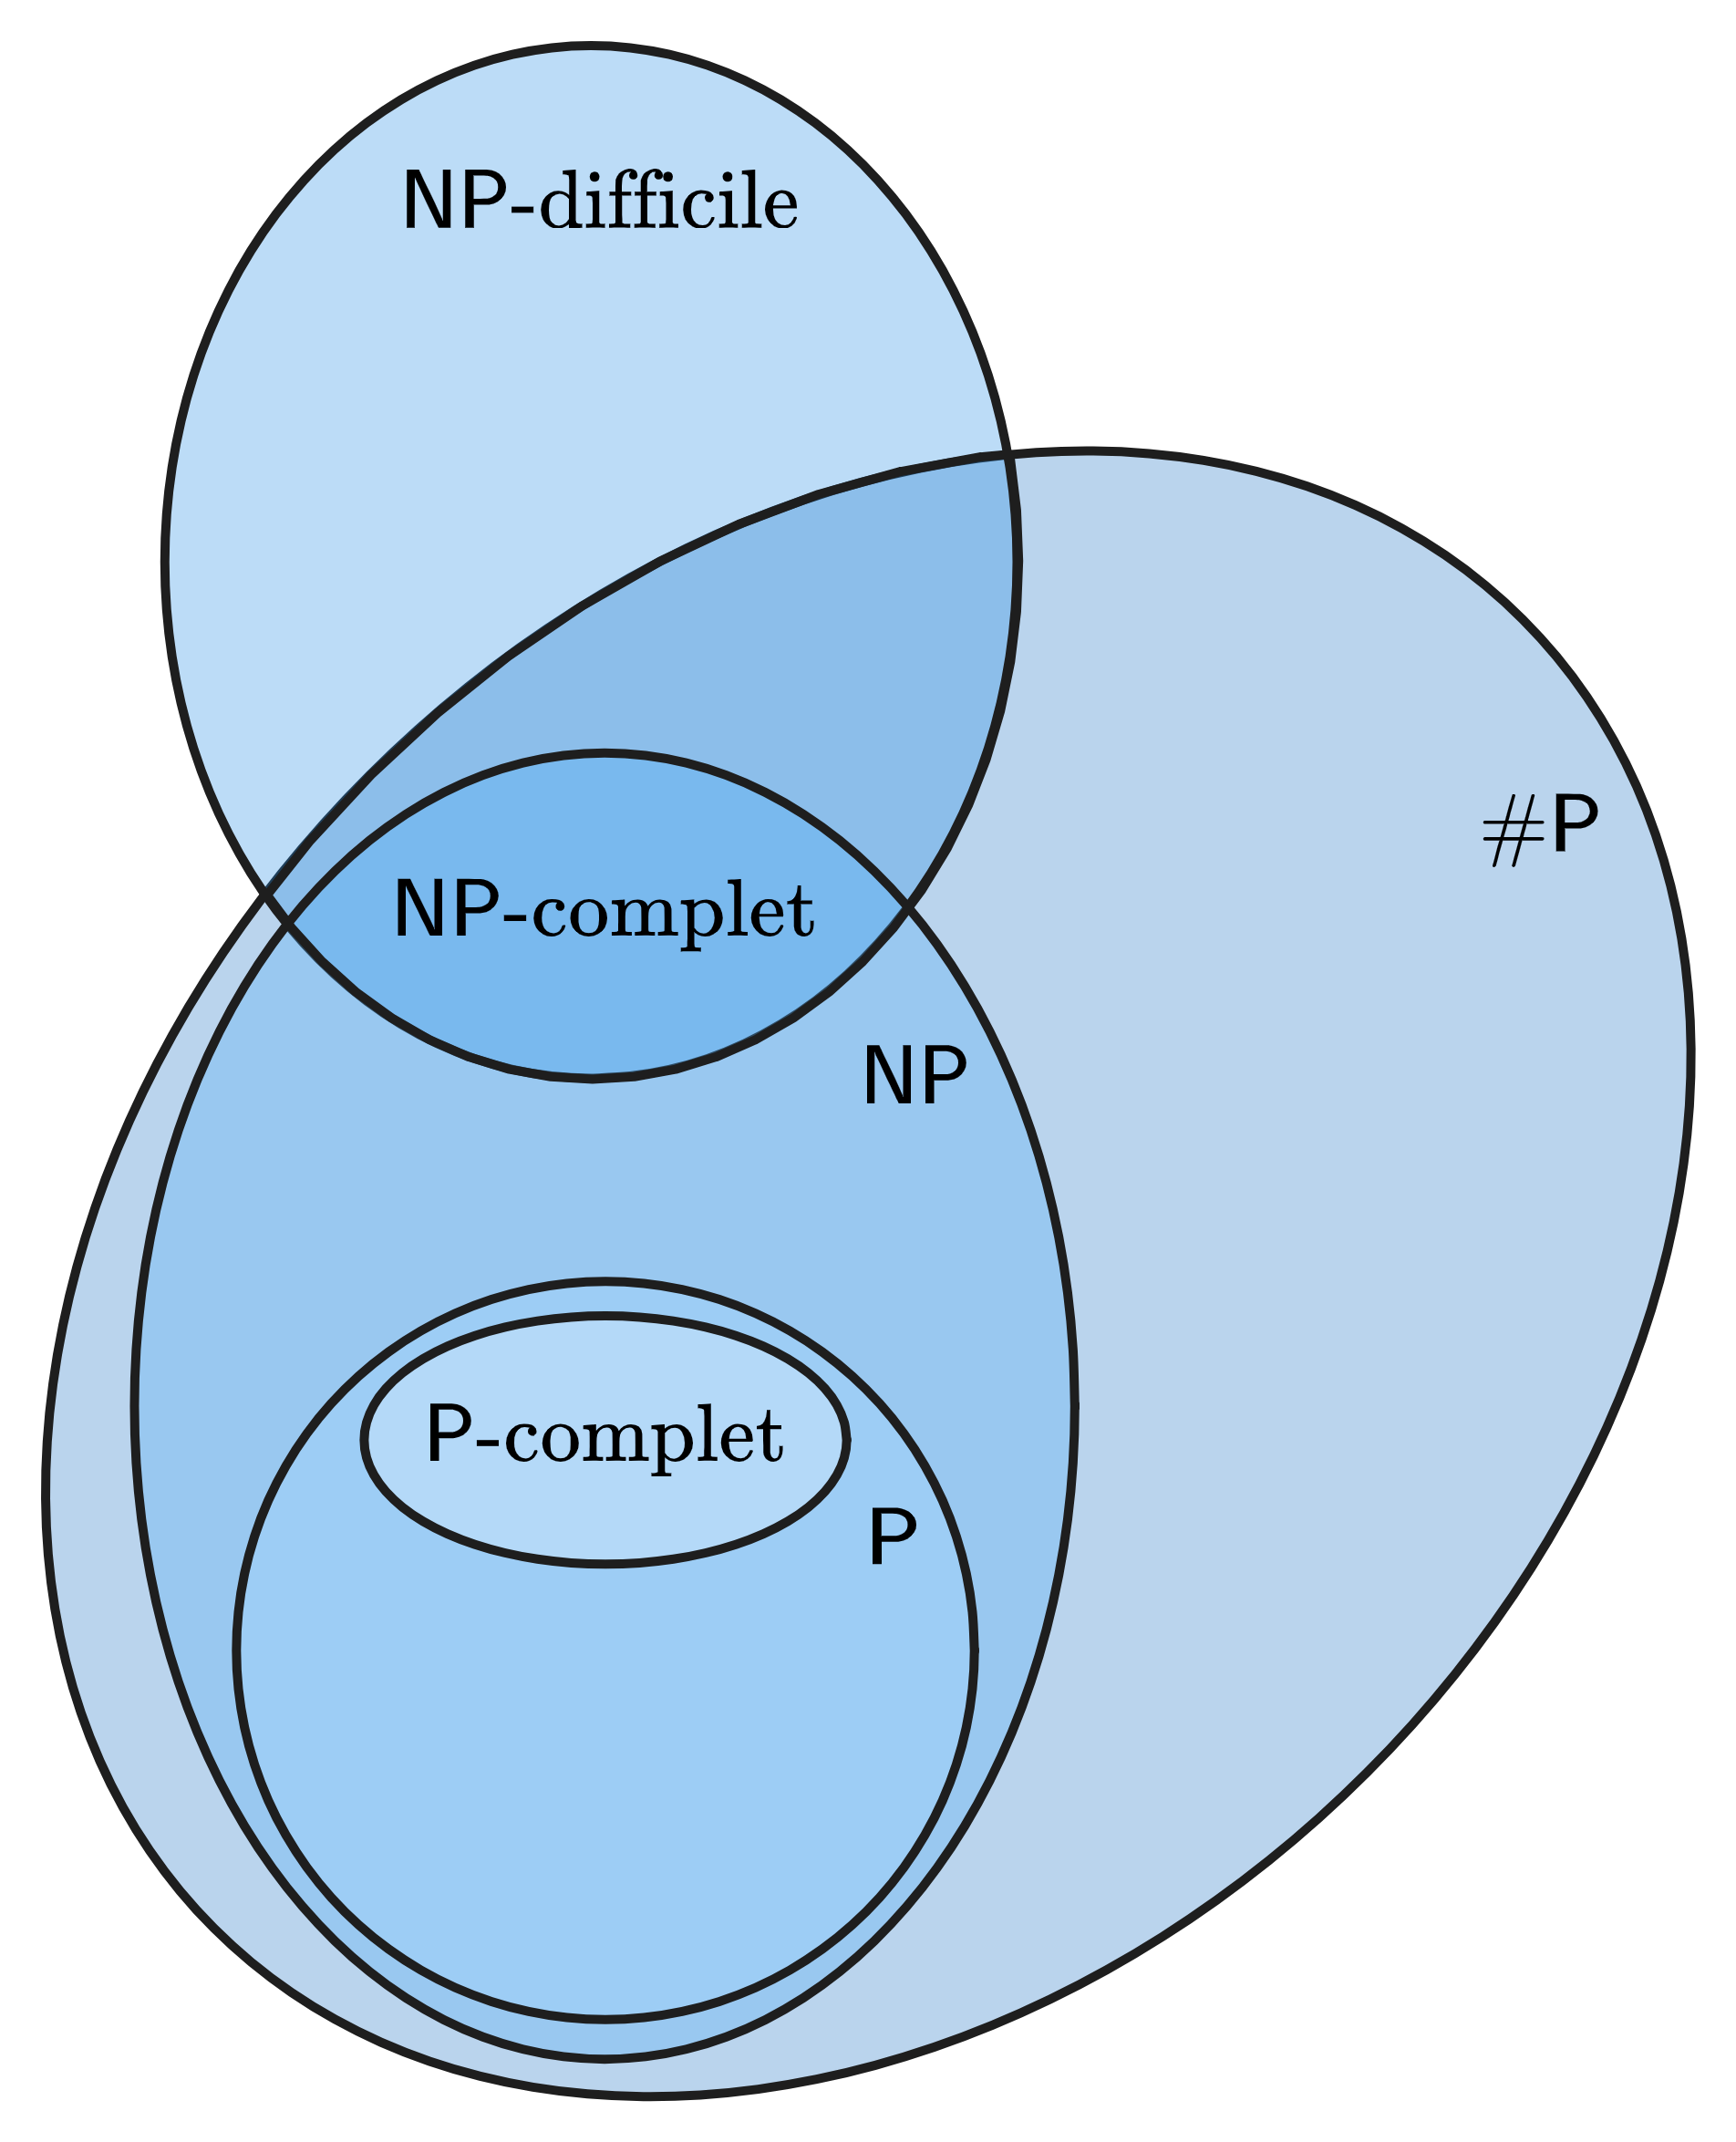
\includegraphics[width=0.4\textwidth]{figures/complexity-classes.png}
    \caption[Classes de complexité]{Classes de complexité.}
    \label{fig:complexity-classes}
\end{figure}

L'importance des problèmes \textsf{\#P} au sein de la théorie de la complexité s'observe entre autres par le théorème de Toda~\cite{todaPPHardPolynomialTime1991}. Ce résultat marquant montre que tous les problèmes de la hiérarchie polynomiale \textsf{PH} peuvent être résolus en temps polynomial avec un oracle résolvant instantanément les problèmes \textsf{\#P}. La hiérarchie polynomiale généralise les classes de complexité \textsf{P}, \textsf{NP} et \textsf{co-NP} en capturant les classes de problèmes exprimés par une alternance de quantificateurs d'existence ($\exists$) ou d'universalité ($\forall$) (voir la définition~\ref{def:classe-np} pour un exemple contenant un seul quantificateur d'existence). Ainsi, la hiérarchie \textsf{PH} est comprise dans la classe de complexité $\textsf{P}^{\textsf{\#P}}$, c'est-à-dire les problèmes résolubles avec un oracle \textsf{\#P}. Comme la hiérarchie polynomiale contient de nombreux problèmes importants, ce théorème suggère l'incroyable puissance des problèmes de comptage.

\begin{subtheorem}{Théorème de Toda}{toda}
    La hiérarchie polynomiale \textsf{PH} est contenue dans $\textsf{P}^{\textsf{\#P}}$.
\end{subtheorem}

% \textcolor{mydarkred}{\textit{https://www.cs.cornell.edu/~sabhar/chapters/ModelCounting-SAT-Handbook-prelim.pdf}}

% L'ordinateur quantique boulverse le domaine de la complexité classique. En effet, la thèse de Church-Turing, stipulant qu'un algorithme est calculable si et seulement s'il est calculable par une machine de Turing, ne prend pas en compte les processus physiques. Le principe de Church-Turing-Deustch généralise la thèse de Church-Turing en énoncçant qu'un dispositif de calcul universel peut simuler n'importe quel processus physique. \textcolor{mydarkred}{\textit{Enlever?}}

L'ordinateur quantique bouleverse le domaine de la complexité classique. Les problèmes autrefois intraitables deviennent potentiellement résolubles efficacement à l'aide d'algorithmes quantiques. Deux nouvelles classes de complexité font alors leurs apparitions pour décrire les problèmes résolubles à l'aide de matériel informatique quantique. La classe \textsf{BQP} généralise la classe \textsf{BPP}, pour « temps polynomial probabiliste à erreur bornée », c'est-à-dire la classe de problèmes résoluble avec une probabilité d'erreur inférieure à $1/3$, pour les ordinateurs quantiques. De plus, la classe de complexité \textsf{QMA}, pour « Merlin Arthur Quantique » se définit par rapport à la classe \textsf{BQP} de manière analogue à la classe \textsf{NP} pour la classe \textsf{P}. La théorie de la complexité quantique étudie les classes de complexité quantiques dans l'objectif de déterminer les problèmes où les algorithmes quantiques comportent un avantage par rapport aux algorithmes classiques. Ce mémoire avance la recherche dans cette direction en étudiant la performance des algorithmes quantiques en comparaison avec les algorithmes classiques.

% Entre, le principe de Church-Turing-Deutsch fût proposée comme une version plus forte de la thèse de Church-Turing en utilisant les lois de la physique. 

% \textcolor{mydarkred}{\textit{Définir les problèmes de décision et de comptage ainsi que les classes de complexité de manière plus formelle (alphabet, )? Changer $B(x,y)$ par $xBy$?}}

% \textcolor{mydarkred}{\textit{Expliquer plus le théorème de Cook-Levin.}}

% \textcolor{mydarkred}{\textit{Discuter des relations entre les classes de complexité définies.}}

% \textcolor{mydarkred}{\textit{Church-Turing-Deutch}}
% \textcolor{mydarkred}{\textit{Parler des problèmes d'optimisation combinatoire.}}

% \textcolor{mydarkred}{\textit{Ajouter une figure sur les classes de complexité.}}
% \textcolor{mydarkred}{\textit{Classe PP}}
% \textcolor{mydarkred}{\textit{Classes de complexité quantique}}

%-----------------------------------------------------------------------------%

\section{Satisfaisabilité booléenne}
\label{sec:satisfaisabilite-booleenne}

\begin{comment}
\subsection*{Plan}

\begin{enumerate}
    \item Introduire SAT
    \item Énumérer certaines applications de ce problème
    \item Faire le lien entre le problème de décision SAT et le problème de comptage SAT
    \item Introduire NAE3SAT et 1in3SAT
    \item Énoncer la réduction entre NAE3SAT/1in3SAT et 3SAT
    \item Introduire la transition de phase critique de ces problèmes
    \item Expliquer pourquoi prendre la version positive de ces problèmes n'est pas un problème
    \item Parler du comptage des problèmes SAT
    \item Introduire la transition de phase critique de ces problèmes
\end{enumerate}

\subsection*{Références}

1. Moore, Cristopher, and Stephan Mertens, The Nature of Computation (Oxford, 2011; online edn, Oxford Academic, 17 Dec. 2013), https://doi.org/10.1093/acprof:oso/9780199233212.001.0001, accessed 19 July 2024.

2. Arora, S. and Barak, B. Computational Complexity: A Modern Approach. (Cambridge University Press, Cambridge, 2009). doi:10.1017/CBO9780511804090.

3. Achlioptas, D., Chtcherba, A., Istrate, G. and Moore, C. The phase transition in 1-in-k SAT and NAE 3-SAT. Proceedings of the Annual ACM-SIAM Symposium on Discrete Algorithms (2001) doi:10.1145/365411.365760.
\end{comment}

Le problème de \textit{satisfaisabilité booléenne} ou problème SAT est particulièrement important dans la théorie de la complexité. Montré comme \textsf{NP}-complet par le théorème de Cook-Levin~\cite{cookComplexityTheoremprovingProcedures1971,levinUniversalSequentialSearch1973}, il fut à la base de la définition de \textsf{NP}-complétude et du problème $\textsf{P} \stackrel{?}{=} \textsf{NP}$. Celui-ci est aussi couramment utilisé dans la preuve de réductions de problèmes au sein de la classe de complexité \textsf
{NP}. Le problème SAT a une multitude d'applications, comme le diagnostic des fautes d'un circuit logique ou la planification en intelligence artificielle~\cite{marques-silvaPracticalApplicationsBoolean2008}, en partie grâce à la facilité de formuler ces applications à l'aide de formules propositionnelles.

Une \textit{formule propositionnelle}, ou une expression booléenne, est un ensemble de variables booléennes, $x_{i} \in \set{\textsc{\texttt{FAUX}}, \textsc{\texttt{VRAI}}}$, reliées par des opérateurs booléens de conjonctions (\textsc{\texttt{OU}}, $\lor$), de disjonctions (\textsc{\texttt{ET}}, $\land$) ainsi que de négation (\textsc{\texttt{NON}}, $\neg$).  Un \textit{littéral} désigne dans ce contexte une variable booléenne ou sa négation. Par exemple, l'expression $(x_{1} \land x_{2}) \lor \neg x_{3}$ est une formule booléenne composée des variables $x_{1}$, $x_{2}$ et $x_{3}$, ainsi que des littéraux $x_{1}$, $x_{2}$ et $\neg x_{3}$. Notons que l'équivalence $\textsc{\texttt{FAUX}} \leftrightarrow 0$ et $\textsc{\texttt{VRAI}} \leftrightarrow 1$ est utilisée dans ce mémoire par commodité.

Un problème SAT se décrit par une formule propositionnelle. Résoudre le problème consiste à déterminer s'il existe une combinaison de variables qui rend la formule logiquement vraie, c'est-à-dire tel que l'évaluation de celle-ci donne 1. Une telle formule est alors dite satisfaisable.

\begin{maindefinition}{Problème SAT}{probleme-sat}
    Soit une constante $n \geq 1$ et une formule propositionnelle $\varphi(x_{1}, x_{2}, \dots, x_{n})$ où $x_{i} \in \set{ 0, 1 }$.  Existe-t-il une assignation des variables $x_{1}, x_{2}, \dots, x_{n}$ telle que $\varphi$ soit satisfaisable, c'est-à-dire que $\varphi(x_{1}, x_{2}, \dots, x_{n})=1$?
\end{maindefinition}

Dans l'étude du problème SAT, les formules propositionnelles sont souvent exprimées en \textit{forme normale conjonctive} (« Conjunctive Normal Form ») (CNF). On parle alors de formules CNF. Celles-ci consistent en une conjonction d'une ou de plusieurs \textit{clauses}, où une clause est une disjonction d'un ou plusieurs littéraux. Cela implique que toute clause doit contenir au moins un littéral évaluant à 1 pour que la formule soit satisfaisable. Toute formule propositionnelle peut être réécrite en forme normale conjonctive en utilisant les lois de l'algèbre booléenne.

\begin{example}{Problème SAT}{probleme-sat}
    La formule CNF
    \begin{equation*}
        \varphi(x_{1}, x_{2}, x_{3}) = (x_{1} \lor x_{3}) \land (\neg x_{1} \lor x_{2} \lor \neg x_{3}) 
    \end{equation*}
    est satisfaisable car $\varphi(1,0,0) = (1 \lor 0) \land (\neg 1 \lor 0 \lor \neg 0) = 1$. Au contraire, la formule CNF
    \begin{equation*}
        \varphi(x_{1})= (x_{1}) \land (\neg x_{1})
    \end{equation*}
    n'est pas satisfaisable car $\varphi (x_{1}) = 0$ peu importe le choix de $x_{1}$.
\end{example}

% \textcolor{mydarkred}{\textit{Tables de vérité?}}

Le problème kSAT constitue un cas spécial du problème SAT, où le nombre de littéraux appartenant à chaque clause d'une formule CNF est restreint à $k$ littéraux au maximum. Notons que le problème kSAT est trivial pour $k=1$, résoluble en temps linéaire pour $k=2$~\cite{kromDecisionProblemClass1967}, et \textsf{NP}-complet pour $k \geq 3$~\cite{karpReducibilityCombinatorialProblems1972}. Surprenamment, les problèmes de comptage correspondant, \#2SAT et \#3SAT, appartiennent tous les deux à la classe \textsf{\#P}-complet~\cite{valiantComplexityEnumerationReliability1979}. Ainsi, compter le nombre de solutions à un problème \textsf{NP}-complet peut être difficile même s'il est possible de trouver une solution efficacement.

Dans ce mémoire, deux variantes de 3SAT seront portées à l'étude: le problème Pas-Tous-Égaux 3SAT (« Not-All-Equal 3-Satisfiability ») (NAE3SAT) et le problème 1-dans-3 3SAT (« One-in-Three 3-Sastisfiability ») (1-in-3SAT). 
Comme le problème SAT, ces problèmes appartiennent aussi à la classe de complexité \textsf{NP}-complet. Les versions monotones de ces problèmes, où la négation de variables n'est pas permise, sont étonnamment aussi \textsf{NP}-complet par le théorème de dichotomie de Schaefer~\cite{schaeferComplexitySatisfiabilityProblems1978}. Ces problèmes de décision peuvent être associés aux problèmes de comptage \#NAE3SAT et \#1-in-3SAT de la classe de complexité \textsf{\#P}.

\begin{maindefinition}{Problème NAE3SAT}{probleme-nae3sat}
    Soit une formule CNF $\varphi(x_{1}, x_{2}, \dots, x_{n})$ pour laquelle chaque clause $C$ contient au maximum 3 littéraux. Existe-t-il une assignation des variables $x_{1}, x_{2}, \dots, x_{n}$ telle que $\varphi$ soit satisfaisable tout en s'assurant que tous les littéraux de chaque clause $C$ ne soient pas égaux?
\end{maindefinition}

Notons qu'un problème NAE3SAT peut être décrit par un problème 3SAT. Soit une formule CNF $f$ exprimant un problème 3SAT. Une formule CNF $g$, représentant le problème NAE3SAT associé à $f$, est construite en transformant chaque clause $(x \lor y \lor z)$ de $f$ en $(x \lor y \lor z) \land (\neg x \lor \neg y \lor \neg z)$. Cette nouvelle contrainte renforce alors la condition supplémentaire, c'est-à-dire que les littéraux de chaque clause ne peuvent être tous égaux. Cette relation illustre bien une symétrie cachée derrière le problème NAE3SAT; chacune des variables possèdent en moyenne la même probabilité d'être vraie ou fausse.

\begin{maindefinition}{Problème 1-in-3SAT}{probleme-1in3sat}
    Soit une formule CNF $\varphi(x_{1}, x_{2}, \dots, x_{n})$ pour laquelle chaque clause $C$ contient au maximum 3 littéraux. Existe-t-il une assignation des variables $x_{1}, x_{2}, \dots, x_{n}$ telle que $\varphi$ soit satisfaisable tout en s'assurant qu'exactement un littéral de chaque clause $C$ soit logiquement vrai?
\end{maindefinition}

De la même façon que pour le problème NAE3SAT, le problème 1-in-3SAT se transforme en un problème 3SAT en transformant chaque clause $(x \lor y \lor z)$ en $(x \lor y \lor z) \land (x \lor \neg y \lor \neg z) \land (\neg x \lor y \lor \neg z) \land (\neg x \lor \neg y \lor z) \land (\neg x \lor \neg y \lor \neg z)$, de manière à encoder la contrainte additionnelle du problème 1-in-3SAT.

% \textcolor{mydarkred}{\textit{Parler du nombre de solutions.}}

%-----------------------------------------------------------------------------%

\section{Intraitabilité, approximation et optimisation}
\label{sec:intractabilite-approximation-et-optimisation}

\begin{comment}
\subsection*{Plan}

\begin{enumerate}
    \item Expliquer le concept d'intractabilité
    \item Montrer la difficulté de résoudre des problèmes computationnels de manière exacte
    \item Expliquer les advantages des méthodes approximatives (temps polynomial, applications réelles)
    \item Introduire rigoureusement le concept d'approximation
\end{enumerate}

\subsection*{Références}

Subhash Khot. Inapproximability of NP-complete Problems, Discrete Fourier Analysis, and Geometry. In Proceedings of the International Congress of Mathematicians 2010 (ICM 2010)
\end{comment}

Les problèmes algorithmiques des classes de complexité \textsf{NP}-difficile et \textsf{\#P}-difficile sont considérés comme intraitables en raison de leur complexité intrinsèque. En effet, il est improbable qu'un algorithme puisse résoudre exactement ces problèmes en temps polynomial. Par exemple, bien que certaines instances du problème SAT contenant plus d'un million de variables sont résolubles efficacement, d'autres instances de moins d'un millier de variables ne peuvent être résolus par les solveurs de pointe~\cite{froleyksSATCompetition20202021}. Cette difficulté s'accentue pour le problème \#SAT, où même une centaine de variables peut s'avérer trop complexe. 

L'intraitabilité de tels problèmes mène alors à un paradigme différent; Sachant qu'il est irréaliste de résoudre certains problèmes exactement, est-ce qu'il est possible de trouver une solution approximative de manière efficace? L'exactitude des solutions est alors sacrifié pour une performance accrue.

Les problèmes de décision ne possédant que deux solutions, oui ou non, il n'est pas possible de fournir une solution approximative. Un \textit{problème d'optimisation}, défini en conjonction à un problème de décision, est alors une notion plus adéquate pour incorporer la notion d'approximation. Ces problèmes ne cherchent plus à trouver la solution optimale, mais plutôt à obtenir une réponse suffisamment près de la valeur optimale. Un exemple de problème d'optimisation, particulièrement étudié dans le domaine de l'optimisation quantique en raison de sa simplicité d'implémentation sur du matériel informatique quantique, est le problème de coupe maximum (­« Maximum Cut ») (Max-Cut). Ce problème cherche une coupe séparant les sommets d'un graphe en deux ensembles complémentaires tel que le nombre d'arêtes séparant les deux ensemble soit maximal. Le problème Max-Cut étant \textsf{NP}-complet, il est difficile d'obtenir une coupe optimale, mais une coupe sous-optimale peut possiblement être trouvée efficacement.

Un problème d'optimisation $\Pi$ est constitué d'un ensemble d'instances valides $I_{\Pi}$, où chaque instance $x \in I_{\Pi}$ possède un ensemble de solutions faisables $S_{\Pi}(x)$. Une fonction objectif $\text{obj}_{\Pi}$, aussi nommée fonction de coût ou de perte, quantifie la qualité d'une solution approximative $y$ de $x$ en lui assignant un nombre réel. En conséquence, résoudre approximativement un problème d'optimisation correspond à minimiser ou maximiser la fonction de coût. Une mesure de succès fréquemment utilisée, autant classiquement que quantiquement, est le \textit{rapport d'approximation},
\begin{equation}
    \alpha(x, y) = \frac{\text{obj}_{\Pi}(x, y)}{\text{OBJ}_{\Pi}(x)} \,,
\end{equation}
où $\text{OBJ}_{\Pi}(x) = \min_{y} \text{obj}_{\Pi} (x, y)$. Ce type de problème est formalisé sous le nom de problème d'optimisation \textsf{NP}, mais une définition détaillée est évitée ici par simplicité. Bien que les algorithmes d'approximation heuristiques offrent fréquemment de bons résultats, ceux-ci ne possèdent aucune garantie quant à la qualité de ces solutions.

Pour pallier ce problème, des algorithmes approximatifs avec garantis sont définis en fonction de deux paramètres: la tolérance $\varepsilon$ et la confiance $\delta$. La tolérance indique l'erreur multiplicative maximale de l'approximation et la confiance indique la probabilité de succès de l'algorithme. Ce couple de paramètres est souvent utilisés pour décrire les algorithmes approximatifs.

Un \textit{algorithme d'approximation de tolérance $\varepsilon$} pallie ce problème en garantissant une solution optimale à une erreur multiplicative près~\cite{vaziraniApproximationAlgorithms2003}. Pour un problème de minimisation $\Pi$, cet algorithme $f$ produit une solution $s$ pour toutes instances $x \in I_{\Pi}$ tel que $f_{\Pi}(x, y) \leq \varepsilon(\lvert x \rvert ) \cdot \text{OBJ}(x)$ où $\lvert  x \rvert $ est la taille de l'instance et $\varepsilon \geq 1   $. Cette définition peut être détendue en permettant à l'algorithme de produire une telle solution avec une certaine probabilité. Cette variante, l'\textit{algorithme d'approximation randomisé de tolérance $\varepsilon$}, introduit des concepts pertinents pour le chapitre~\ref{cha:echantillonnage-quasi-uniforme-comptage-approximatif-randomise}.

% \textcolor{mydarkred}{\textit{What is $f$?}}

\begin{subtheorem}{Algorithme d'approximation randomisé}{algorithme-approximation-randomise}
    Un algorithme d'approximation randomisé de tolérance $\varepsilon$ pour un problème de minimisation $\Pi$ est un algorithme aléatoire prenant en entrée une instance $x \in D_{\Pi}$ et une tolérance $\varepsilon$ et qui produit une solution $y \in S_{\Pi}(x)$ tel que
    \begin{equation*}
        \mathrm{ Pr } [f_{\Pi}(x, y) \leq \varepsilon(\lvert x \rvert ) \cdot \text{OBJ}(x)] \geq \frac{1}{2}
    \end{equation*}
    en temps polynomial.
\end{subtheorem}

Ces algorithmes se généralisent facilement pour un problème de maximisation.
En relaxant la condition d'exactitude, il est attendu qu'un gain en possible en terme d'efficacité. Cependant, cela n'est pas toujours aussi clair. Il existe en effet certains problèmes où trouver une solution approximative en haut d'un certain rapport d'approximation demeure intraitable tel le problème de couverture par ensembles~\cite{lundHardnessApproximatingMinimization1994}. Les algorithmes d'approximation s'appliquent aussi aux problèmes de comptage, tel que présenté à la section~\ref{sec:comptage-approximatif-randomise}.

%-----------------------------------------------------------------------------%

\section{Comptage de modèles}
\label{sec:comptage-de-modeles}

\begin{comment}
\subsection*{Plan}

\begin{enumerate}
    \item Décrire les résultats actuels en terme de comptage exact et approximatif
    \item Énumérer les algorithmes et les solveurs modernes (DPLL, \textit{survey propagation}, \textit{belief propagation})
    \item Mentionner les meilleures bornes sur les problèmes de comptage
    \item https://arxiv.org/pdf/2002.06879
    \item Lien avec la fonction de partition
\end{enumerate}

\subsection*{Références}

1. Wahlström, M. A Tighter Bound for Counting Max-Weight Solutions to 2SAT Instances. in Parameterized and Exact Computation (eds. Grohe, M. and Niedermeier, R.) 202–213 (Springer, Berlin, Heidelberg, 2008). doi:10.1007/978-3-540-79723-419.

2. Sinclair, A. and Jerrum, M. Approximate counting, uniform generapportn and rapidly mixing Markov chains. Information and Computation 82, 93–133 (1989).
\end{comment}

% est-il possible de préciser sa complexité dans le pire des cas? Une quantité signifiante de travaux s'intéresse à cette question.

Sachant désormais que le comptage est un problème difficile, comment résoudre celui-ci? Le comptage des solutions d'une formule propositionnelle est spécifiquement connu dans la littérature sous le nom de \textit{comptage de modèles}. De nombreuses méthodes, autant exactes qu'approximatives, ont été développées pour sa résolution~\cite{biereHandbookSatisfiability2009}. 

Les méthodes exactes attaquent généralement le problème en explorant exhaustivement l'espace des solutions possibles, de manière similaire à l'algorithme de Davis-Putnam-Logemann-Loveland (DPLL) pour les problèmes SAT~\cite{davisMachineProgramTheoremproving1962}. Les algorithmes de recherche locale pour SAT, tel l'algorithme WalkSAT, peuvent aussi être étendus pour résoudre \#SAT. Toutefois, les solveurs les plus performants actuellement sont basés sur les réseaux de tenseurs, un object mathématique provenant du domaine de la matière condensée~\cite{kourtisFastCountingTensor2019, dudekEfficientContractionLarge2020, dudekParallelWeightedModel2021}. Ces réseaux sont utiles dans de nombreux autres domaines et sont d'ailleurs utilisés dans ce travail pour la simulation de circuit quantique et font donc l'objet de l'annexe~\ref{ann:simulation-circuits-quantiques-avec-reseaux-de-tenseurs}. Bien que différents développements accentuent la taille des systèmes résolubles exactement, les solveurs ont de la difficulté à trouver l'ensemble de solutions de l'espace de recherche. 

Les méthodes approximatives allègent ce problème à l'aide d'heuristiques fournissant des estimations avec ou sans garanties. Plusieurs applications du comptage ne nécessitent pas un résultat exact; distinguer la différence entre $10^{30}$ et $10^{30}+1$ solutions n'est pas toujours pertinent. L'algorithme de Stockmeyer, qui approxime le nombre de solutions à un facteur deux avec un nombre polynomial d'appels à un oracle \textsf{NP} en s'appuyant sur les fonctions de hachage, fut un pas majeur pour le comptage approximatif~\cite{stockmeyerComplexityApproximateCounting1983}. Plusieurs modifications ont propulsé le domaine vers des performances accrues de sorte que la majorité des méthodes modernes se basent effectivement sur les fonctions de hachage. Cependant, une méthode alternative due à Jerrum, Valiant et Vazirani utilise plutôt la relation entre l'échantillonnage aléatoire de solutions et le comptage approximatif pour résoudre le problème. Malgré l'originalité de cette idée, la recherche dans cette direction s'est estompée en raison de la difficulté de l'échantillonnage de solutions avec les conditions nécessaires. Ce travail relance cette possibilité en pourvoyant une nouvelle façon d'échantillonner avec les algorithmes variationnels quantiques. Une discussion approfondie est présentée au chapitre~\ref{cha:echantillonnage-quasi-uniforme-comptage-approximatif-randomise}.

Les avancées en physique, tel les réseaux de tenseurs, présentent des avantages pour le comptage de modèle, mais l'inverse est aussi vrai. Le problème du comptage est intimement reliée au domaine de la mécanique statistique. En effet, déterminer la fonction de partition d'un système à température nulle est en réalité équivalent à un problème de comptage~\cite{timmeCountingComplexDisordered2009}. Considérons la fonction de partition $Z$ pour un Hamiltonien $H$ où l'énergie fondamentale est fixée à $E_{0} = 0$,
\begin{equation}
    Z = \sum_{i} e^{-\beta E_{i}} \,,
\end{equation}
où $\beta = \frac{1}{k_{b} T}$, $k_{B}$ est la constante de Boltzmann et $T$ est la température. Dans la limite $T \to 0$, les seuls termes non-nuls de la somme sont $e^{-\beta E_{0}}$, c'est-à-dire les termes associés aux états fondamentaux du système. Ainsi, pour un système dégénéré de $N_{0}$ états fondamentaux, la fonction de partition devient $Z = N_{0}$. Calculer la fonction de partition correspond ainsi à déterminer le nombre d'états fondamentaux.

Le développement du calcul quantique a aussi mené à de fructueux aboutissements. L'algorithme de comptage quantique prend avantage de l'algorithme de Grover et de l'algorithme d'estimation de phase quantique pour approximer le nombre de solutions à l'aide de $(\sqrt{\frac{N}{M}})$ itérations, où $M$ est le nombre de solutions, de taille exponentielle pour les problèmes SAT et $N$ est le nombre d'états possibles~\cite{brassardQuantumAmplitudeAmplification2002, wieSimplerQuantumCounting2019, aaronsonQuantumApproximateCounting2020}. Le nombre d'itérations nécessaires profite ainsi d'un gain quadratique par rapport à la complexité optimale classique de $O(\frac{N}{M})$.

Notons que dans tous les cas, le comptage de solutions aux formules CNF, l'objet de ce travail, ne s'effectue jamais en temps polynomial. Même les approches approximatives nécessitent un nombre exponentiel d'opérations, indiquant davantage la difficulté de ce problème.


% \textcolor{mydarkred}{\textit{Model counting!}}
% \textcolor{mydarkred}{\textit{Hashing based}}
% \textcolor{mydarkred}{\textit{JVV}}
% \textit{}
% \textcolor{mydarkred}{\textit{Permanent}}

% \textcolor{mydarkred}{\textit{Quantum counting?}}

% \textcolor{mydarkred}{\textit{https://www.scottaaronson.com/papers/apxcount.pdf}}

% \textcolor{mydarkred}{\textit{https://www.cs.cornell.edu/~sabhar/chapters/ModelCounting-SAT-Handbook-prelim.pdf}}

% \textcolor{mydarkred}{\textit{https://www.cs.toronto.edu/~meel/Papers/handbook-chapter.pdf}}

% \textcolor{mydarkred}{\textit{Partition function}}

%-----------------------------------------------------------------------------%

\section{Transitions de phase}
\label{sec:transitions-de-phase}

\begin{comment}
\subsection*{Plan}

\begin{enumerate}
    \item Expliquer les différentes transitions de phase et leurs intuitions
    \item Décrire l'objectif des algorithmes classiques locaux et globaux, comme le "belief propagation" ou le "survey propagation"
    \item Expliquer brièvement où se situe VQCount par rapport à ça
\end{enumerate}

\subsection*{Références}

1. Watrous, J. Quantum Computational Complexity. Preprint at https://doi.org/10.48550/arXiv.0804.3401 (2008).

2. Mézard, M. and Montanari, A. Information, Physics, and Computation. (Oxford University Press, Oxford, New York, 2009).

2. https://www.sciencedirect.com/science/article/pii/S0378437109010656

3. Survey propagation: An algorithm for satisfiability - Braunstein - 2005 - Random Structures amp; Algorithms - Wiley Online Library. https://onlinelibrary.wiley.com/doi/abs/10.1002/rsa.20057.
\end{comment}

La complexité d'une instance aléatoire d'un problème \textsf{NP} n'est pas toujours équivalente. En réalité, certaines instances sont résolubles en temps polynomial, alors que d'autres sont intraitables. Les discussions autour des classes de complexité s'intéressent principalement à la complexité dans le pire des cas pour décrire la difficulté inhérente d'un problème. Cependant, certaines instances peuvent posséder une complexité inférieure, pouvant alors être pris en avantage par certains algorithmes. 

Pour les problèmes SAT, la difficulté d'une instance aléatoire est grandement dépendante sur le rapport $\alpha = \frac{m}{n}$, où $m$ est le nombre de clauses et $n$ est le nombre de variables. Intuitivement, cette difficulté provient de l'ajout de contraintes au problème sous la forme de clauses. Plus surprenamment, la complexité d'une telle instance suit une transition de phase nommée \textit{transition de phase critique}. En effet, il existe une valeur critique $\alpha_{c}$ où les instances du problème SAT passe de satisfaisable à insatisfaisable dans la limite asymptotique de $n$. La difficulté du problème SAT est maximale juste avant cette transition. Pourquoi est-ce le cas?

Plusieurs autres transitions de phase existent avant la transition critique telle qu'illustré à la figure~\ref{fig:transitions-de-phase}. Ces transitions, similairement aux transitions de phase du modèle d'Ising, correspondent à des changements dans l'organisation de l'ensemble des solutions. Pour décrire cette réorganisation, une mesure de similarité est nécessaire pour comparer les différentes entrées au problème SAT. La \textit{distance de Hamming} entre deux chaînes de bits de même taille correspond au nombre de positions dans les chaînes où les bits correspondants diffèrent. 


Avant la première transition de phase, la \textit{transition de phase de regroupement}, toutes les solutions d'une instance du problème SAT sont situées au sein du même amas, chacune à une distance d'Hamming polynomiale selon la taille de l'instance. \textcolor{mydarkred}{\textit{Compléter.}}

% \textit{transition de phase de congélation}

\begin{figure}[h]
    \centering
    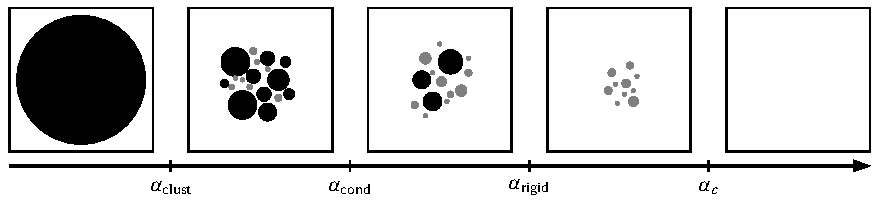
\includegraphics[width=1\textwidth]{figures/phase-transitions.pdf}
    \caption[Transitions de phase du problème SAT]{Schéma des transitions de phase du problème SAT selon le rapport du nombre de clauses au nombre de variables $\alpha$. Les transitions de phases illustrées sont la transition de regroupement $\alpha_{\text{clust}}$, la transition de condensation $\alpha_{\text{cond}}$, la transition de congélation $\alpha_{\text{rigid}}$ et la transition de satisfaisabilité $\alpha_{c}$.}
    \label{fig:transitions-de-phase}
\end{figure}

Les approches locales semblent échouer à la transition de condensation, alors que la difficulté du problème SAT semble provenir de la transition de congélation. La transition de phase critique pour NAE3SAT est situé à $\alpha_{c} \approx 2.1$~\cite{achlioptasPhaseTransition1ink2001} et à $\alpha_{c} \approx 2/3$~\cite{raymondPhaseDiagram1in32007} pour 1-in-3SAT. Les instances du problème \#1-in-3SAT près du seuil critique appartiennent à la catégorie des problèmes bloqués. Les problèmes \#P dans ce régime sont parmi les plus difficiles~\cite{zdeborovaStatisticalPhysicsHard2008}.

% \textcolor{mydarkred}{\textit{Pourquoi transition dynamique?}}

% \textcolor{mydarkred}{\textit{Parler du nombre de solutions.}}

% \textcolor{mydarkred}{\textit{Locked problems.}}


% \textcolor{mydarkred}{\textit{Voir papier de stefanos fast counting, plus d'informations et de références.}}

% \textcolor{mydarkred}{\textit{Algorithme local vs global}}

~\cite{dyerMarkovChainsIndependent2000}
~\cite{barthelClusteringAnalysisGroundstate2004}

\begin{comment}
\end{comment}

\chapter{Échantillonnage quasi aléatoire et comptage approximatif}

\subsection*{Plan}

\begin{enumerate}
    \item Énoncer brièvement l'algorithme de JVV pour introduire la section
    \item Re-mentionner l'importance du comptage approximatif (en autres en comparaison avec le comptage exact)
    \item Mentionner les concepts nécessaires pour l'algorithme de JVV (auto-réductibilité, échantillonnage quasi aléatoire, comptage approximatif)
\end{enumerate}
\subsection*{Références}

%-----------------------------------------------------------------------------%

\section{Auto-réductibilité}
 
\begin{comment}
\subsection*{Plan}

\begin{enumerate}
    \item Introduire les concepts d'auto-réductibilité
\end{enumerate}

\subsection*{Références}

1. Hemaspaandra, L. A. The Power of Self-Reducibility: Selectivity, Information, and Approximation. Preprint at https://doi.org/10.48550/arXiv.1902.08299 (2019).

\subsection*{Brouillon}

Introduction de "Autoreducibility" par Trakhtenbrot.

Introduction de "Self-reducibility" par Schnorr et Meyer/Paterson.

Survey paper de Balcázar, Selke, Allender.

Explication simple par Hemaspaandra.
\end{comment}

L'auto-réductibilité (\textit{self-reducibility}) est un concept complexe, essentiel à la compréhension du calcul et de la complexité, découlant de l'introduction de la réduction automatique (\textit{autoreducibility})~\cite{trakhtenbrotAutoreducibility1970}. Ces concepts sont particulièrement importants dans le contexte de génération aléatoire et du comptage approximatif, ainsi que pour la réduction entre le problème de décision et les problèmes de recherche.

La \textit{réduction automatique} peut être introduite informellement de la manière suivante:

\begin{subdefinition}{Réduction automatique}{auto-reductibilite}
    Un problème algorithmique est dit \textit{automatiquement réductible} s'il peut être résolu par un algorithme résolvant d'autres instances du même problème, sans que l'algorithme puisse interroger l'instance particulière qu'il cherche à résoudre.
\end{subdefinition}

Les problèmes automatiquement réductibles contiennent de l'information d'appartenance redondante, c'est-à-dire qu'il existe une structure dans l'ensemble de problèmes pouvant être exploitée pour simplifier le calcul d'une instance donnée. Ainsi, un algorithme peut résoudre une instance en utilisant l'information redondante présente dans d'autres instances, évitant ainsi les requêtes directes à l'instance en question. Connaître la solution à une autre problème peut alors aider la résolution du problème initial. 

\textcolor{mydarkred}{\textit{Exemple: Halting problem?}}

Pour discuter de la génération aléatoire et le comptage approximatif, l'\textit{auto-réductibilité descendante}, une forme limité de la réduction automatique, est une définition plus adéquate. En effet, cette condition est nécessaire à l'application de l'algorithme JVV. Informellement, on peut définir celle-ci comme:

\begin{maindefinition}{Auto-réductibilité descendante}{auto-reductibilite-informel}
    Un problème algorithmique est dit \textit{auto-réductible descendant} s'il peut être résolu grâce à un algorithme résolvant des instances de taille strictement inférieure.
\end{maindefinition}

\textcolor{mydarkred}{\textit{Quelle est vraiment la différence entre auto-reducibility et self-reducibility?}}

Cette propriété s'éclaircit en prenant le problème SAT comme exemple, qui s'avéra particulièrement utile dans la compréhension de l'algorithme JVV à la section~\ref{sec:algorithme-jvv}. L'auto-réductibilité appliquée au problème de satisfaisabilité s'exprime facilement avec la relation suivante:

\begin{relation}{Auto-réductibilité pour les problèmes SAT}{auto-reductibilite-sat}
    Soit une constante $n \geq 1$ et une formule propositionelle $\varphi(x_{1}, x_{2}, \dots, x_{n})$ où $x_{i} \in \set{ 0, 1 }$. Alors,
    \begin{equation*}
        \varphi(x_{1}, x_{2}, \dots, x_{n}) = 1 \iff \varphi(x_{1}=0, x_{2}, \dots, x_{n}) = 1 \lor \varphi(x_{1}=1, x_{2}, \dots, x_{n}) = 1
    \end{equation*}
\end{relation}

Cette relation implique que l'ensemble de solutions d'une instance donnée peut être exprimée comme l'ensemble de solutions de deux instances plus petite du problème. \textcolor{mydarkred}{\textit{Élaborer...}}

Plus précisément, le problème SAT est décrit comme une auto-réductibilité à longueur décroissante 2-disjonctive. Ici, 2-disjonctive fait référence à une formule propositionnelle dans une disjonction ($\lor$) d'une conjonction ($\land$) d'au plus deux variables. Longueur décroissante, ou descendante, signifie que l'algorithme résout des instances de taille strictement inférieure.

Une définition rigoureuse de l'auto-réductibilité peut aussi être pratique.

\begin{maindefinition}{Auto-réductibilité descendante}{auto-reductibilite-formel}
    Soit $\Sigma^{*}$ un ensemble fixé et fini encodant les instances d'un problème ainsi que leurs solutions. Soit $R \subseteq \Sigma^{*} \times \Sigma^{*}$ une relation binaire assignant à chaque instance de problème $x \in \Sigma^{*}$ un ensemble de solutions $R(x) = \set{ y \in \Sigma^{*} \mid xRy }$. Une relation $R \subseteq \Sigma^{*} \times \Sigma^{*}$ est auto-réductible si et seulement si
    \begin{enumerate}
        \item il existe une fonction calculable en temps polynomial $g \in \sigma^{*} \to \mathbb{N}$ tel que $xRy \implies \lvert y \rvert = g(x)$;
        \item il existe une fonction calculable en temps polynomial $\psi \in \Sigma^{*} \times \Sigma^{*} \to \Sigma^{*}$ et $\sigma \in \Sigma^{*} \to \mathbb{N}$ satifaisant
        \begin{align*}
            & \sigma(x)=O(\log |x|) \\
            & g(x)>0 \Rightarrow \sigma(x)>0 \quad \forall x \in \Sigma^{\star} \\
            & |\psi(x, w)| \leqslant|x| \quad \forall x, w \in \Sigma^{\star}
        \end{align*}
        et tel que, pour tout $x \in \Sigma^{*}, y=y_1 \ldots y_n \in \Sigma^{*}$, 
        \begin{equation*}
            \left\langle x, y_1 \ldots y_n \right\rangle \in R \Leftrightarrow \left\langle \psi \left( x, y_1 \ldots, y_{\sigma(x)} \right), y_{\sigma(x)+1} \ldots y_n \right\rangle \in R
        \end{equation*}
    \end{enumerate}
\end{maindefinition}




%-----------------------------------------------------------------------------%

\section{Échantillonnage quasi uniforme}

\begin{comment}
\subsection*{Plan}

\begin{enumerate}
    \item Introduire les FPAUS
    \item Introduire la distance en variation totale et la non-uniformité
\end{enumerate}

\subsection*{Références}
\end{comment}

\begin{maindefinition}{Échantillonneur quasi uniforme pleinement polynomial (FPAUS)}{fpaus}
    Un échantillonneur quasi uniforme pour un ensemble de solutions $S \subseteq \Sigma^{*} \times \Sigma^{*}$, où $S$ représente la relation entre les instances d'un problème $x$ et de ses solutions $y \in  S(x)$, est un algorithme aléatoire prenant en entrée une instance $x \in \Sigma^{*}$ et une tolérance d'échantillonnage $\delta > 0$ et qui génère une solution $y \in S(x)$ tel que
    \begin{equation*}
        \lVert Y - U \rvert_{TV} \leq \delta 
    \end{equation*}
    où $Y$ est la distribution de probabilité de $y$ et $U$ est la distribution de probabilité uniforme sur $S(x)$. Si l'algorithme s'exécute en temps borné par un polynomial en $\lvert x \rvert$ et en $\ln (\delta^{-1})$, on parle d'échantillonneur quasi uniforme pleinement polynomial.
\end{maindefinition}

\textcolor{mydarkred}{\textit{Changer la définition pour celle du papier de JVV?}}

%-----------------------------------------------------------------------------%

\section{Comptage approximatif}

\begin{comment}
\subsection*{Plan}

\begin{enumerate}
    \item Introduire les FPRAS
    \item Introduire les algorithmes de comptage classique connus (ex.: Stockmeyer et JVV)
\end{enumerate}

\subsection*{Références}

1. Stockmeyer, L. The complexity of approximate counting. in Proceedings of the fifteenth annual ACM symposium on Theory of computing 118–126 (Association for Computing Machinery, New York, NY, USA, 1983). doi:10.1145/800061.808740.
\end{comment}

\begin{maindefinition}{Schéma d'approximation aléatoire pleinement polynomial (FPRAS)}{fpras}
    Un schéma d'approximation aléatoire pour un problème de comptage $f: \Sigma^{*} \to \mathbb{N}$ est un algorithme aléatoire prenant en entrée une instance d'un problème $x \in \Sigma^{*}$ et une tolérance d'erreur $\varepsilon > 0$ et qui génère un nombre $N \in \mathbb{N}$ tel que, pour toute instance $x$,
    \begin{equation*}
        \mathrm{ Pr }\left[(1+\varepsilon)^{-1} f(x) \leq N \leq (1+\varepsilon)f(x)\right] \geq \frac{3}{4} .
    \end{equation*}
    Si l'algorithme s'exécute en temps borné par un polynomial en $\lvert x \rvert$ et $\varphi^{-1}$, alors on parle de schéma d'approximation aléatoire pleinement polynomial.
\end{maindefinition}

%-----------------------------------------------------------------------------%

\section{Algorithme de Jerrum-Valiant-Vazirani}
\label{sec:algorithme-jvv}

\begin{comment}
\subsection*{Plan}

\begin{enumerate}
    \item Introduire le but de l'algorithme de JVV
    \item Vulgariser l'algorithme de JVV
    \item Introduire rigoureusement l'algorithme de JVV
    \item Rajouter l'algorithme complet sous forme de pseudo-code.
\end{enumerate}

\subsection*{Références}

1. Jerrum, M. R., Valiant, L. G. and Vazirani, V. V. Random generation of combinatorial structures from a uniform distribution. Theoretical Computer Science 43, 169–188 (1986).
2. Huber, M. Exact sampling and approximate counting techniques. in Proceedings of the thirtieth annual ACM symposium on Theory of computing 31–40 (Association for Computing Machinery, New York, NY, USA, 1998). doi:10.1145/276698.276709.
\end{comment}

\begin{figure}[h]
    \centering
    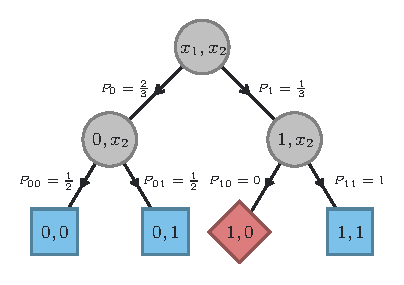
\includegraphics[width=0.5\textwidth]{figures/jvv-algorithm.pdf}
    \caption{}
    \label{fig:jvv-algorithm}
\end{figure}

\chapter{Algorithmes variationnels quantiques}
\label{cha:algorithmes-variationnels-quantiques}
%-----------------------------------------------------------------------------%

\begin{comment}
\subsection*{Plan}

\begin{enumerate}
    \item Décrire les algorithmes variationels en général (algorithmes hybrides)
    \item Expliquer les objectifs de ces algorithmes
    \item Expliquer les avantages (exemple: algorithmes à court-terme, qubits bruités, NISQ)
    \item Expliquer la chronologie avec les QAOA
    \item Expliquer comment est-ce qu'on peut utiliser ceux-ci comme générateur pour l'algorithme JVV.
    \item Pourquoi est-ce que QAOA est une approche non-locale?
\end{enumerate}
    
\subsection*{Références}

1. Cerezo, M. et al. Variational quantum algorithms. Nat Rev Phys 3, 625–644 (2021).

2. Bharti, K. et al. Noisy intermediate-scale quantum (NISQ) algorithms. Rev. Mod. Phys. 94, 015004 (2022).
\end{comment}

En général, le comptage est un problème ardu. En acceptant une solution approximative, la complexité de ce problème peut être déplacée à l'échantillonnage quasi uniforme de solutions à ce problème grâce à l'algorithme de JVV. Toutefois, la construction d'un tel générateur n'a pas encore été évoquée. En fait, la majorité des solutionneurs de problème \textsf{\#P} ne se basent pas sur l'échantillonnage en raison de la difficulté d'obtenir une distribution uniforme composée de solutions. Est-ce que le calcul quantique peut offrir une méthode efficace pour la génération uniforme de solutions?

Les \textit{algorithmes variationnels quantiques} (« Quantum Variational Algorithms ») (VQA) sont des algorithmes hybrides, c'est-à-dire composés d'une partie quantique et d'une partie classique, conçus pour exploiter les avantages du calcul quantique tout en profitant de la puissance des algorithmes classiques~\cite{cerezoVariationalQuantumAlgorithms2021}. Ces algorithmes ont émergés comme la stratégie dominante pour atteindre l'avantage quantique avec le matériel informatique quantique actuel, connu sous le nom des ordinateurs quantiques bruités de taille intermédiaire (« Noisy Intermediate-Scale Quantum ») (NISQ). En effet, les algorithmes quantiques possédant un avantage par rapport aux algorithmes classiques sont présentement hors d'atteinte pour les ordinateurs quantiques du moment en raison de la taille des systèmes nécessaires et des erreurs causées par le bruit. Le concept derrière des VQA s'inspire des méthodes d'apprentissage automatique pour résoudre des problèmes d'optimisation combinatoire avec des circuits de faible profondeur sans se soucier de la correction des erreurs des qubits. Un état quantique initial facile à préparer est évolué unitairement avec un circuit quantique paramétré et la valeur moyenne d'une fonction de coût est estimé par de multiples mesures du circuit dans une base appropriée. Les paramètres du circuit sont alors ajustés itérativement avec un optimiseur classique pour minimiser la fonction de coût et ainsi préparer un état près d'une superposition des solutions du problème. Cette approche limite les inconvénients causés par le bruit en raison de l'utilisation de circuits paramétrés limitant la taille des circuits utilisés. Ainsi, les VQA sont une option possible pour la résolution de problèmes d'échantillonnage de l'algorithme de JVV.

% Un circuit quantique paramétré est d'abord préparé sur un ordinateur quantique et un optimiseur classique modifie itérativement les paramètres de ce circuit pour minimiser la fonction de coût d'un problème à l'aide des mesures du circuit préparé. 

Cet chapitre introduit d'abord l'algorithme adiabatique quantique à la section~\ref{sec:algorithme-adiabatique-quantique}, fondant la base théorique de QAOA. Après avoir détaillé QAOA à la section~\ref{sec:algorithme-quantique-d'optimisation-approximative}, différentes variantes de QAOA sont explorées, tel comme sa généralisation, l'ansatz quantique  opérateur alternées, et une variante de celle-ci utilisant le forçage de Grover à la section~\ref{sec:ansatz-quantique-a-operateurs-alternants}. Finalement, deux propriétés de QAOA sont explorés, c'est-à-dire l'initialisation et l'optimisation des paramètres du circuit quantique à la section~\ref{subsec:configuration-des-parametres} et le biais d'échantillonnage à la section~\ref{sec:echantillonnage-et-biais}.

% \textcolor{mydarkred}{\textit{Importance des heuristiques quantiques (voir qaoa (2e version) paper)}}

%-----------------------------------------------------------------------------%

\section{Algorithme adiabatique quantique}
\label{sec:algorithme-adiabatique-quantique}

\begin{comment}
\subsection{Plan}

\begin{enumerate}
    \item QAA est adiabatique alors que QAOA est contre-adiabatique.
\end{enumerate} 
\end{comment}

Le \textit{théorème adiabatique}, introduit par Born et Fock~\cite{bornBeweisAdiabatensatzes1928}, peut être énoncé simplement comme suit:

\begin{subtheorem}{Théorème adiabatique}{theoreme-adiabatique}
    Un système physique demeure dans son état propre instantané si une perturbation donnée agit sur lui suffisamment lentement et s'il y a un intervalle significatif entre la valeur propre et le reste du spectre de l'hamiltonien.
\end{subtheorem}

Bien que différentes versions de ce théorème furent rigoureusement formulées~\cite{albashAdiabaticQuantumComputing2018}, une version approximative de celui-ci, proposée par Messiah~\cite{messiahQuantumMechanics1999} et rectifiée par Amin~\cite{aminConsistencyAdiabaticTheorem2009}, est présentée ici dans l'objectif d'élucider les mécanismes du théorème. Un système quantique, décrit par un hamiltonien dépendant du temps $H(t)$, évolue selon l'équation de Schrödinger

% , en commençant par Kant en 1950~\cite{katoAdiabaticTheoremQuantum1950},

\begin{align*}
   i \hbar \frac{\partial \ket{\psi(t)}}{\partial t} = H(t) \ket{\psi} \,.
\end{align*}

Considérons ici que l'hamiltonien $H(t)$ peut s'écrire sous la forme $H(t) = \tilde{H}(s)$, où $s=t/T \in [0,1]$ est le temps adimensionnel, de manière que $T$ contrôle le taux de variation dans le temps de $H(t)$. Soit $\ket{\varepsilon_{j} (s)}$ les états propres instantanés de $\tilde{H}(s)$ avec énergie $\varepsilon_{j}$ (potentiellement dégénérée) tel que

\begin{equation}
   \tilde{H}(s) \ket{\varepsilon_{j}(s)} = \varepsilon_{j}(s) \ket{\varepsilon_{j}(s)} \,,
\end{equation}

où $\varepsilon_{j}(s) < \varepsilon_{j+1}(s) \ \forall j,s$ et $j \in \set{ 0, 1, 2, \dots }$. L'approximation adiabatique indique qu'un état initial préparé dans un des états propres instantanés $\ket{\varepsilon_{j}(0)}$ demeure dans le même état propre instantané $\ket{\varepsilon_{j}(t)}$ à une phase globale près si $\varepsilon_{i}(s) - \varepsilon_{j}(s) \neq  0$ et

\begin{equation}
    T \gg \max_{s \in [0,1]} \frac{\lvert \braket{ \varepsilon_{i}(s) | \partial_{s} \tilde{H}(s) | \varepsilon_{j}(s) } \rvert }{\lvert \varepsilon_{i}(s) - \varepsilon_{j}(s) \rvert^{2} } \ \forall j \neq i \,.
\end{equation}

% \textcolor{mydarkred}{\textit{Rajouter une intuition et un lien avec le théorème.}}

L'approximation adiabatique est souvent utilisée à partir de l'état fondamental $\ket{\varepsilon_{0}(t)}$, menant à la définition du gap spectral entre l'état fondamental et le premier état excité du système $\Delta(s) = \varepsilon_{1}(s) - \varepsilon_{0}(s)$. Généralement, le maximum de $\braket{ \varepsilon_{i}(s) | \partial_{s} \tilde{H}(s) | \varepsilon_{j}(s)}$ est de l'ordre d'une valeur propre typique de $\tilde{H}$ et petit. Le minimum du carré de l'inverse du gap spectral $\Delta$ constitue alors un critère pratique pour quantifier le temps nécessaire à l'évolution adiabatique.

% \textcolor{mydarkred}{\textit{Reformuler et faire attention aux symboles.}}

L'\textit{algorithme adiabatique quantique} (« Quantum Adiabatic Algorithm ») (QAA), introduit par Farhi, Gutmann et Sipser~\cite{farhiQuantumComputationAdiabatic2000}, emploie un ordinateur quantique physique pour la résolution de problèmes d'optimisation combinatoire en se basant sur le théorème adiabatique quantique. Pour ce faire, le système physique est initialement préparé dans l'état fondamental d'un hamiltonien de forçage $H_{D}$ facile à construire et dont l'état fondamental est simple à trouver. La solution du problème, encodée dans l'état fondamental de l'hamiltonien de problème $H_{P}$, est alors obtenue en transitionnant de l'état fondamental de l'hamiltonien $H_{D}$ à l'état fondamental de l'hamiltonien $H_{P}$ par une évolution adiabatique. Plus précisément, l'hamiltonien du système s'écrit comme


\begin{equation}
\label{eq:chemin-adiabatique}    
    \tilde{H}(s) = \left(1-s\right) H_{D} + s H_{P} \,.
\end{equation}

Ainsi, en présumant que le gap spectral entre l'état fondamental et l'état excité est non-nul, la solution du problème est toujours obtenue à partir de l'état fondamental obtenu si l'évolution, donnée par l'opérateur $U(t) = e^{-i \int_{0}^{1} \tilde{H}(s) ds}$, est suffisamment lente tel que garantit par le théorème adiabatique quantique. Si le temps d'évolution est trop petit, une \textit{transition diabatique}, c'est-à-dire une transition de l'état fondamental à un état excité, peuvent empêcher l'évolution adiabatique.

\begin{figure}[ht!]
    \centering
    \begin{subfigure}{.48\textwidth}
        \centering
        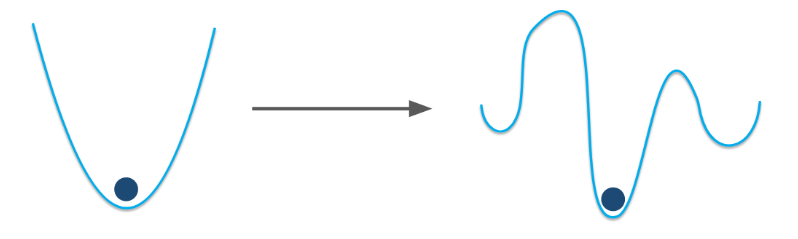
\includegraphics[width=1\textwidth]{figures/algorithme-adiabatique-quantique.png}
        \caption{}
        \label{fig:algorithme-adiabatique-quantique-1}
    \end{subfigure}
    \begin{subfigure}{.48\textwidth}
        \centering
        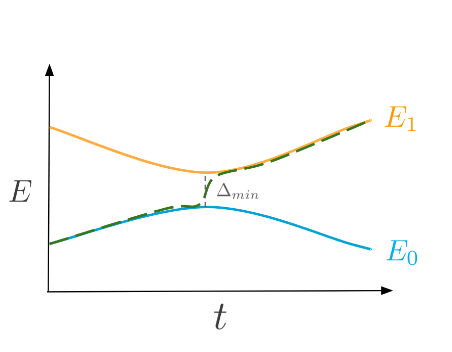
\includegraphics[width=1\textwidth]{figures/algorithme-adiabatique-quantique-2.png}
        \caption{}
        \label{fig:algorithmne-adiabatique-quantique-2}
    \end{subfigure}
    \caption[Algorithme adiabatique quantique]{\textcolor{mydarkred}{\textit{Refaire les figures.}}}
    \label{fig:algorithme-adiabatique-quantique}
\end{figure}

Typiquement, le gap spectral est non-nul~\cite{farhiQuantumComputationAdiabatic2000}, mais cela n'est pas suffisant pour rendre l'algorithme utile comme ce gap doit être assez grand pour limiter le temps d'évolution. Le gap spectral peut être suffisamment grand pour permettre une évolution adiabatique dans un temps réaliste pour certains problèmes, mais ce n'est pas toujours possible~\cite{altshulerAndersonLocalizationMakes2010}. Une alternative consiste à trouver un compromis entre le temps d'évolution et la proximité de l'état final avec l'état fondamental espéré. Le choix du chemin adiabatique utilisé pour transitionner de $H_{D}$ à $H_{P}$ peut aussi différer de l'équation~\ref{eq:chemin-adiabatique} dans l'objectif de maximiser le gap au long du chemin et donc minimiser le temps d'évolution~\cite{nishimoriExponentialEnhancementEfficiency2017, hormoziNonstoquasticHamiltoniansQuantum2017}.

L'algorithme adiabatique quantique se place au sein du \textit{calcul adiabatique quantique}, qui regroupe différentes méthodes similaires. Un autre membre de ce groupe est le \textit{recuit quantique} qui représente généralement l'emploi de QAA dans un environnement bruité, menant ainsi à une version plus réaliste sans contrainte d'adiabaticité ou d'universalité. Cet algorithme partage plusieurs similitudes avec l'algorithme quantique d'optimisation approximative qui seront explorées dans les prochaines sections. 

% \textcolor{mydarkred}{\textit{https://arthurpesah.me/assets/pdf/introduction-quantum-annealing.pdf}}

%-----------------------------------------------------------------------------%

\section{Algorithme quantique d'optimisation approximative}
\label{sec:algorithme-quantique-d'optimisation-approximative}

\begin{comment}
\subsection*{Plan}
    
\begin{enumerate}
    \item Expliquer l'histoire et le lien avec le recuit quantique
\end{enumerate}

\subsection*{Références}

1. Farhi, E., Goldstone, J. and Gutmann, S. A Quantum Approximate Optimization Algorithm. Preprint at https://doi.org/10.48550/arXiv.1411.4028 (2014).

2. Kadowaki, T. and Nishimori, H. Quantum annealing in the transverse Ising model. Phys. Rev. E 58, 5355–5363 (1998).

3. Finnila, A. B., Gomez, M. A., Sebenik, C., Stenson, C. and Doll, J. D. Quantum annealing: A new method for minimizing multidimensional functions. Chemical Physics Letters 219, 343–348 (1994).

4. Farhi, E. et al. A Quantum Adiabatic Evolution Algorithm Applied to Random Instances of an NP-Complete Problem. Science 292, 472–475 (2001).

5. Farhi, E., Goldstone, J., Gutmann, S. and Sipser, M. Quantum Computation by Adiabatic Evolution. Preprint at https://doi.org/10.48550/arXiv.quant-ph/0001106 (2000).

6. Parler la adiabatic quantum computation https://arxiv.org/abs/1611.04471
\end{comment}

Bien que le calcul adiabatique quantique soit utilisé pour résoudre les problèmes d'optimisation combinatoire, le temps nécessaire pour une évolution adiabatique constitue un facteur limitant pour de nombreux problèmes. L'\textit{algorithme quantique d'optimisation approximative} (« Quantum Approximate Optimization Algorithm ») (QAOA)~\cite{farhiQuantumApproximateOptimization2014} propose alors une alternative, sous la forme d'un algorithme variationnel quantique, discrétisant l'évolution continue de QAA. Bien que cette approche s'éloigne de l'évolution adiabatique, celle-ci prend avantage des transitions diabatiques entre l'état fondamental et les états excités pour réduire le temps d'évolution. L'optimisation des paramètres du circuit quantique paramétré permet de naviguer efficacement l'espace de Hilbert pour atteindre une bonne solution approximative. En fait, QAOA est contre-adiabatique et non seulement adiabatique, signifiant que des raccourcis à l'adiabacité sont possibles~\cite{wurtzCounterdiabaticityQuantumApproximate2022}

% QAOA trouve des bonnes approximations pour de nombreux problèmes d'optimisation, comme les problèmes de coupe maximal
% De nombreuses extensions à QAOA ont été présentés au cours des dernières années~\cite{blekosReviewQuantumApproximate2024}.+

% \textcolor{mydarkred}{\textit{Applications}}

% D'abord, l'algorithme tel qu'initialement proposé est introduit. Une discussion plus poussée détaille ensuite les composantes importantes de l'algorithme et un lien avec le calcul adiabatique quantique est présenté pour finir.

%-----------------------------------------------------------------------------

\subsection{Description de l'algorithme}
\label{subsec:description-algorithme}

\begin{comment}
subsection*{Plan}
    
\begin{enumerate}
    \item Décrire le \textit{Quantum Approximate Optimization Algorithm}
    \item QAOA sees the whole graph?
    \item avantage vs les algorithmes classiques?
\end{enumerate}

\subsection*{Références}

1. Farhi, E., Goldstone, J. and Gutmann, S. A Quantum Approximate Optimization Algorithm. Preprint at https://doi.org/10.48550/arXiv.1411.4028 (2014).
\end{comment}

Étant une idée prometteuse pour les applications des ordinateurs quantiques, l'algorithme quantique d'optimisation approximative a mené à une quantité incroyable de travaux dans les précédentes années. Ainsi, pour simplifier la compréhension de ce concept, l'algorithme original, dû à Farhi, Goldstone et Gutmann~\cite{farhiQuantumApproximateOptimization2014}, est d'abord présenté.

QAOA repose sur deux différents hamiltoniens: l'hamiltonien de problème, ou de phase, $H_{P}$ et l'hamiltonien de forçage, ou de mélange, $H_{D}$. L'hamiltonien de problème est formulé de façon à encoder la solution, potentiellement dégénérée, du problème d'optimisation combinatoire dans son état fondamental. Pour ce faire, celui-ci est défini en fonction de la fonction de coût $C$ de l'instance du problème: $H_{P}\ket{x} = C(x)\ket{x}$. $H_{P}$ prend typiquement la forme de l'hamiltonien du modèle d'Ising. L'hamiltonien de forçage, quant à lui, est donné par

\begin{equation}
    \label{eq:x-drive}
    H_{D}^{X} = \sum_{i=1}^{n} X_{i} \,,
\end{equation}

où $X_{i}$ est l'opérateur de Pauli $X$ appliqué sur le qubit $i$ d'un système à $n$ qubits. $H_{D}^{X}$ est construit de manière à induire de l'interférence et ainsi permettre l'exploration de l'espace de Hilbert. 

Par définition, l'hamiltonien $H_{p}$ est diagonal dans la base computationnelle, alors que l'hamiltonien $H_{D}$ comprend des termes hors diagonaux de sorte que ceux-ci ne commutent pas entre eux. Deux opérations unitaires paramétrées sont définies à partir des hamiltoniens $H_{P}$ et $H_{D}$: l'opérateur de problème $U_{P}(\gamma) = e^{-i \gamma H_{P}}$ ainsi que l'opérateur de forçage $U_{D}(\beta) = e^{-i \beta H_{D}}$, où $\gamma$ et $\beta$ sont des paramètres réels. L'opérateur $U_{P}$ représente une rotation de phase, paramétrisée par $\gamma$, des états de la base computationnelle en fonction de leur énergie donné par $H_{P}$. L'opérateur $U_{D}$, paramétrisé par $\beta$, superpose différents états de la base computationnelle ayant précédemment acquis différents facteurs de phase, menant ainsi à de l'interférence.

En tant que VQA, QAOA est un algorithme hybride composé d'un circuit quantique paramétré et d'un optimiseur classique. Le circuit quantique est d'abord préparé dans un état propre de l'hamiltonien de forçage. Pour l'hamiltonien~\ref{eq:x-drive}, un exemple d'état initial possible est dans une superposition égale des états possibles $= \ket{+}^{\otimes n}$. Le produit des opérateurs $U_{D}U_{P}$ est alors appliqué en alternance $p$ fois sur l'état initial $\ket{\psi_{0}}$, donnant l'état suivant:

\begin{equation}
    \label{eq:final-state}
    \ket{\psi(\vec{\gamma}, \vec{\beta})} = \underbrace{U_D(\beta_p) U_P(\gamma_p) \cdots U_D(\beta_1) U_P(\gamma_1)}_{p \text{ fois }} \ket{\psi_{0}} \,,
\end{equation}

où $\vec{\gamma} = (\gamma_{1}, \dots, \gamma_{p})$ et $\vec{\beta} = (\beta_{1}, \dots, \beta_{p})$ sont les paramètres initiaux du circuit. Une fois l'état $\ket{\psi(\vec{\gamma}, \vec{\beta})}$ préparé, la valeur moyenne de l'hamiltonien de problème $H_{P}$ est calculé par des mesures répétées de l'état final dans la base computationnelle:

\begin{equation}
    E_{P} (\vec{\gamma}, \vec{\beta}) = \braket{ \psi(\vec{\gamma}, \vec{\beta}) | H_{P} | \psi(\vec{\gamma}, \vec{\beta}) } \,.
\end{equation}

Comme $H_{P}$ est typiquement une somme d'opérateurs de Pauli, cette valeur moyenne peut être évaluée efficacement en mesurant l'état du circuit préparé\textcolor{mydarkred}{\textit{CITE MIKE AND IKE!}}. L'énergie trouvée quantifie l'optimalité de l'état préparé. Par la suite, une méthode d'optimisation classique continue, comme la descente de gradient stochastique, est employée pour mettre à jour itérativement les paramètres $\gamma$ et $\beta$ du circuit paramétré de manière à minimiser la valeur moyenne $E_{P} (\vec{\gamma}, \vec{\beta})$:

\begin{equation}
    (\vec{\gamma}^{*}, \vec{\beta}^{*}) = \arg \min_{{\vec{\gamma}, \vec{\beta}}} E_{P}(\vec{\gamma}, \vec{\beta}) \,.
\end{equation}

Si l'optimisation aboutit de manière espérée, l'état final $\ket{\psi(\vec{\gamma}^{*}, \vec{\beta}^{*})}$ correspond à une superposition des états fondamentaux de $H_{P}$ et donc aux différentes solutions du problème étudié. Si ce n'est pas le cas, le ratio d'approximation $\alpha$ est utilisé pour décrire la qualité de la solution trouvée comme à la section~\ref{sec:intractabilite-approximation-et-optimisation}:

\begin{equation}
    \alpha_{\vec{\gamma}^{*}, \vec{\beta}^{*}} = \frac{ E_{p} (\vec{\gamma}^{*}, \vec{\beta}^{*})}{\min_{(\vec{\gamma}, \vec{\beta})} E_{p} (\vec{\gamma}, \vec{\beta}) }
\end{equation}

Ce ratio augmente théoriquement avec le nombre de couches $p$ utilisées comme QAOA équivaut à une évolution adiabatique dans la limite $p \to \infty$~\cite{farhiQuantumApproximateOptimization2014}. Notons que pour l'utilisation de QAOA sur des graphes, la valeur de $p$ doit augmenter avec la taille du graphe pour ne pas être limité par la localité de QAOA~\cite{farhiQuantumApproximateOptimization2020}.

L'algorithme se résume par les étapes suivantes, illustrées dans la figure~\ref{fig:qaoa}:

\begin{enumerate}[(1)]
    \item Définition de l'hamiltonien de problème $H_{P}$.
    \item Préparation de l'état initial $\ket{\psi_{0}}$.
    \item Construction du circuit quantique paramétré $\ket{\psi(\gamma, \beta)}$ en appliquant en alternance les opérateurs $U_{P}(\gamma)$ et $U_{D}(\beta)$ $p$ fois.
    \item Calcul de l'énergie $E_{P}$ à travers de mesures dans la base computationnelle.
    \item Optimisation des paramètres $\vec{\gamma}$ et $\vec{\beta}$ à l'aide d'un optimiseur classique minimisant l'énergie $E_{P}$.
\end{enumerate}


\begin{figure}[ht!]
    \centering
    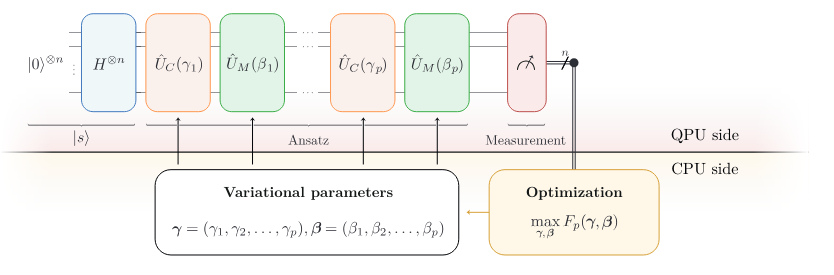
\includegraphics[width=0.7\textwidth]{figures/qaoa.png}
    \caption[Algorithme quantique d'optimisation approximative]{\textcolor{mydarkred}{\textit{Refaire la figure.}}}
    \label{fig:qaoa}
\end{figure}

Décrivons maintenant plus en détails les mécanismes derrière QAOA: la préparation de l'état initial, l'encodage du problème dans un hamiltonien de problème ainsi que le choix de l'hamiltonien de forçage. L'initialisation et l'optimisation des paramètres du circuit est décrit à la section~\ref{subsec:configuration-des-parametres}.

%-----------------------------------------------------------------------------%

\subsubsection{Préparation de l'état initial}
\label{subsec:preparation-de-etat-initial}

Comme QAA, le circuit quantique est initialement préparé dans l'état fondamental de l'hamiltonien de forçage pour garantir le théorème adiabatique. Cependant, la divergence de QAOA du calcul adiabatique implique qu'un autre choix d'état initial peut être choisi. Une alternative consiste à utiliser une solution approximative du problème comme état initial~\cite{eggerWarmstartingQuantumOptimization2021}. 

%-----------------------------------------------------------------------------%

\subsubsection{Encodage du problème}
\label{subsec:encodage-probleme}

\begin{comment}
\subsection*{Plan}

\begin{enumerate}
    \item Introduire la fonction de coût
    \item Introduire le modèle d'Ising et le modèle QUBO
    \item Décrire la transformation d'Ising pour NAE3SAT et 1in3SAT
    \item Prouver la transformation d'Ising pour NAE3SAT et 1in3SAT
\end{enumerate}

\subsection*{Références}

1. Lucas, A. Ising formulations of many NP problems. Frontiers in Physics 2, (2014).
2. MAPPING NP-HARD AND NP-COMPLETE OPTIMISATION PROBLEMS
TO QUADRATIC UNCONSTRAINED BINARY OPTIMISATION PROBLEMS. (CORRECTION DE 1)

\end{comment}

Comment est-ce qu'un problème d'optimisation combinatoire $\varphi(x)$ peut être encodé par un hamiltonien $H_{P}$? D'abord, les entrées $x$ du problème sont caractérisées par une fonction de coût $C(x)$, composés termes de pénalisant les configurations non-valides. Une entrée optimale est associée à un coût nul, alors qu'une entrée non optimale est associée à un coût positif selon sa proximité avec les solutions. Résoudre le problème correspond alors à trouver l'entrée optimale, c'est-à-dire l'entrée $x^{*}$ minimisant la fonction de coût. L'hamiltonien de problème se définit par

\begin{equation}
    H_{P} \ket{x} = C(x) \ket{x}
\end{equation}

Cette équation implique que l'état fondamental de l'hamiltonien $H_{P}$ encode les solutions au problème donné. Un état préparé dans l'état fondamental de $H_{P}$ correspond ainsi à une superposition des solutions au problème $\varphi$. Le modèle d'Ising est fréquemment utilisé pour fournir un hamiltonien décrivant la fonction de coût $C$:

\begin{equation}
    \label{eq:hamiltonien-ising}
    H_P = - \sum_{(i,j) \in E} J_{ij} \sigma_i \sigma_j - \sum_{i \in V} h_i \sigma_i \,,
\end{equation}

où $E$ est l'ensemble d'arêtes, $V$ est l'ensemble de sommets et $\sigma_{i}$ est le spin de la particule $i$. Les constantes $J$ et $h$ représentent respectivement l'interaction entre deux sites et le champ magnétique externe. Le problème d'optimisation quadratique binaire non contraint (« Quadratic Unconstrained Binary Optimization ») (QUBO) permet aussi d'exprimer les fonctions de coût de manière plus générale, en ne les restreignant pas au modèle d'Ising.

\begin{figure}[h]
    \centering
    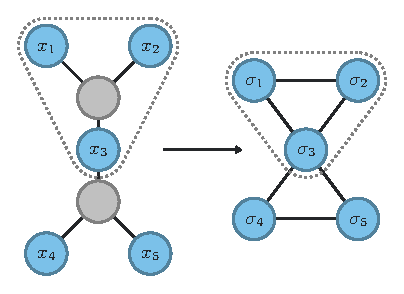
\includegraphics[width=0.55\textwidth]{figures/ising-mapping}
    \caption[Transformation du problème \#NAE3SAT et \#1-in-3SAT au modèle d'Ising]{Exemple de la transformation entre le modèle d'Ising pour NAE3SAT et 1-in-3SAT pour une formule $\varphi$. À gauche, le graphe de facteurs de $\varphi$ avec les sommets de variables (bleus) et de clauses (gris). À droite, le modèle d'Ising correspondant à $\varphi$. Pour 1-in-3SAT, un terme de champ magnétique est ajouté pour favoriser les configurations où chaque clause contienne exactement un variable fixée à 1.}
    \label{fig:transformation-ising}
\end{figure}

Comme trouver l'état fondamental d'un modèle d'Ising constitue un problème \textsf{NP}-complet, il existe alors nécessairement une réduction entre ce problème et les différents problèmes \textsf{NP}-complet. Bien que ces réductions ne sont pas nécessairement évidentes, plusieurs de celles-ci ont été formulées pour le calcul adiabatique quantique~\cite{lucasIsingFormulationsMany2014,lodewijksMappingNPhardNPcomplete2020}. Une réduction intéressante dans notre cas relie le problème positif NAE3SAT au modèle d'Ising antiferromagnétique. Une formule CNF $\varphi$ peut être représentée graphiquement sous la forme d'un graphe bipartie nommé \textit{facteur de graphes}. Dans ce graphe, les clauses et les variables sont représentés sous la forme de sommet alors la présence des variables dans une clause sont représentées à l'aide d'arêtes entre les deux partitions. Considérons pour le moment une seule clause $C = (x_{1} \lor x_{2} \lor x_{3})$ de $\varphi$. En associant chaque variable $x_{i}$ à un spin $\sigma_{i}$ selon la transformation $\sigma_{i} = 1 - 2x_{i}$, cette clause se réduit à un modèle d'Ising en considérant un réseau triangulaire composé des spins $\sigma_{i}$, où chacun de ceux-ci sont reliés aux deux autres spins tels qu'illustré à la figure~\ref{fig:transformation-ising}. L'hamiltonien d'un tel modèle est donné par

\begin{equation}
    H_{P, C} = \sigma_{1}\sigma_{2} + \sigma_{2}\sigma_{3} + \sigma_{3}\sigma_{1}
\end{equation}

Les énergies associées à chaque combinaison possible des spins sont présentés dans le tableau~\ref{tab:energie-nae3sat}, où les spins vers le haut sont représentés par 0 et les spins vers le bas sont représentés par 1. La frustration des spins sur le réseau implique que les seuls états qui ne sont pas dans l'état fondamental sont les états $000$ et $111$. Hors, il s'agit des deux combinaisons ne faisant pas partie de l'ensemble des solutions du problème positif NAE3SAT. L'état fondamental de l'hamiltonien $H_{P, C}$ correspond ainsi bien aux solutions de la clause $C$.

\begin{table*}[h]
    \centering
    \begin{subtable}{0.4\textwidth}
        \centering
        \begin{tabular}{c c}
            \hline
            Entrée & Énergie \\
            \hline
            000 & 3 \\
            001 & -1 \\
            010 & -1 \\
            100 & -1 \\
            011 & -1 \\
            110 & -1 \\
            101 & -1 \\
            111 & 3 \\
            \hline
        \end{tabular}
        \caption{}
        \label{tab:energie-nae3sat}
    \end{subtable}
    % \hspace*{4em}
    \begin{subtable}{0.4\textwidth}
        \centering
        \begin{tabular}{c c}
            \hline
            Entrée & Énergie \\
            \hline
            000 & 0 \\
            001 & -2 \\
            010 & -2 \\
            100 & -2 \\
            011 & 0 \\
            110 & 0 \\
            101 & 0 \\
            111 & 6 \\
            \hline
        \end{tabular}
        \caption{}
        \label{tab:energie-1in3sat}
    \end{subtable}
    \caption{Énergie de chaque entrée dans le modèle d'Ising pour le problème NAE3SAT (a) et 1-in-3SAT (b).}
\end{table*}

La formule est représentable par un modèle d'Ising en appliquant la transformation précédente sur chacune des clauses de la formule, tel qu'illustré à la figure~\ref{fig:transformation-ising}, donnant ainsi l'hamiltonien 

\begin{equation}
    H_{P} = \sum_{C} H_{P, C} \,,
\end{equation}

de manière que chaque clause soit respectée. Ainsi, l'hamiltonien de problème pour NAE3SAT est donné par l'équation~\ref{eq:hamiltonien-ising} avec $J_{ij}=-1$ et $h_{i}=0$. Le problème 1-in-3SAT se transforme au modèle d'Ising en ajoutant pour chaque clause l'hamiltonien

\begin{align*}
   H_{P, C} = \sigma_{1}\sigma_{2} + \sigma_{2}\sigma_{3} + \sigma_{3}\sigma_{1} - \sigma_{1} - \sigma_{2} - \sigma_{3}
\end{align*}

Un champ magnétique externe est ajouté pour imposer la contrainte supplémentaire, c'est-à-dire que toutes les clauses doivent contenir exactement une variable évaluant à vrai. Le tableau~\ref{tab:energie-1in3sat} présente les énergies des configurations pour l'hamiltonien précédent. L'hamiltonien pour le problème 1-in-3SAT est donc donnée par l'équation~\ref{eq:hamiltonien-ising} avec $J_{ij}=-1$ et $h_{i}=1$.

%-----------------------------------------------------------------------------%

\subsubsection{Choix du forçage}

\begin{comment}
\subsection*{Plan}

\begin{enumerate}
    \item Expliquer le but du forçage
    \item Expliquer forçage en X
    \item Expliquer le forçage de Grover
    \item Énumérer les forçages populaires
    \item Est-ce que le mixer doit être un vecteur propre de l'état initial?
\end{enumerate}

\subsection*{Références}
\end{comment}

L'hamiltonien de forçage $H_{D}$ initialement proposé avec QAOA prends son inspiration de l'algorithme adiabatique quantique, en utilisant l'hamiltonien facile à préparer $H_{D}^{X}$. Cela implique que toute la dépendance au problème doit être encodée dans l'hamiltonien de problème $H_{P}$. Comme QAOA n'est pas restreint par cette condition, des opportunités se présentent pour encoder différemment le problème. Par exemple, l'Hamiltonien de forçage peut être utilisé pour restreindre l'espace de Hilbert en prenant en compte la structure du problème. Divers hamiltoniens offrent différentes performances selon le problème étudié. Le choix de forçage demeure encore une question ouverte. 

%-----------------------------------------------------------------------------%

\subsection{Relation avec l'algorithme adiabatique quantique}
\label{subsec:discretisation-qaoa}

\begin{comment}
    \begin{itemize}
        \item Contre-diabacité
        \item Trottérisation
    \end{itemize}
\end{comment}

QAA requiert une évolution continue de l'état, alors que QAOA repose sur l'application de portes quantiques. Pour établir un lien entre QAA et QAOA, l'évolution de l'hamiltonien doit donc être rendu discrète. Pour ce faire, la décomposition de Suzuki-Trotter, donnée par $e^{(A+B)t} = \lim_{n \to \infty} (e^{At / n} e^{Bt / n})^{n}$ pour deux opérateurs $A$ et $B$, est employée. Le premier ordre de cette décomposition permet de discrétiser l'opérateur de l'hamiltonien dépendant du temps $H(t)=(1-\frac{t}{T})H_{D} + \frac{t}{T}H_{P}$ de QAA (voir l'équation~\ref{eq:chemin-adiabatique}), où $t \in [0, T]$, tel que

\begin{equation}
    e^{-i\Delta t H(t)} \approx e^{-i (1 - \frac{t}{T}) H_D \Delta t} e^{-i \frac{t}{T} H_P \Delta t} + O(\Delta t^2) \,,
\end{equation}

où $\Delta t$ est le pas de temps. Ainsi, l'évolution unitaire de QAA peut être émulée avec des portes quantiques en décomposant $U(t) = e^{-i \int_{0}^{T} H(t) dt}$ en séquence de petits pas de temps à l'aide de la formule de Suzuki-Trotter au premier ordre:

\begin{align*}
   U(t) \approx \prod_{k=0}^{t / \Delta t -1} e^{-i H(k \Delta t) \Delta t} = \prod_{k=0}^{t / \Delta t -1} e^{-i (1 - \frac{k \Delta t}{T}) H_{D} \Delta t} e^{- i \frac{k \Delta t}{T} H_{P} \Delta t} \,.
\end{align*}

Ce processus est généralement nommé \textit{évolution adiabatique trottérisée} d'après la décomposition de Suzuki-Trotter. La forme de QAOA est alors retrouvée en remplaçant $(\frac{kt}{T}) \Delta t$ et $(1 - \frac{kt}{T}) \Delta t$ par les paramètres $\gamma$ et $\beta$. Dans la limite $p \to \infty$, la condition adiabatique est satisfaite comme une évolution adiabatique trottérisé est retrouvée. Par contre, pour une profondeur de circuit $p$ finie, plus les paramètres $\gamma$ et $\beta$ est petits, plus les erreurs dues à la décomposition, dites erreurs de Trotter, sont petites. Cependant, cela implique aussi que le temps d'évolution adiabatique $T$ est plus petit et donc que des excitations diabatiques affectent négativement la performance de l'algorithme. Au contraire, si les paramètres sont grands, le temps d'évolution augmente aux dépens de l'impact des erreurs de Trotter. Un compromis entre ces deux facteurs doit être choisi.

%-----------------------------------------------------------------------------%

\section{Ansatz quantique à opérateurs alternants}
\label{sec:ansatz-quantique-a-operateurs-alternants}

\begin{comment}
\subsection*{Plan}

\begin{enumerate}
    \item Décrire le \textit{Quantum Alternating Operator Ansatz}
    \item Décrire \textit{Grover-Mixer Quantum Alternating Operator Ansatz}
\end{enumerate}

\subsection*{Références}

1. Hadfield, S. et al. From the Quantum Approximate Optimization Algorithm to a Quantum Alternating Operator Ansatz. Algorithms 12, 34 (2019).

2. Bärtschi, A. and Eidenbenz, S. Grover Mixers for QAOA: Shifting Complexity from Mixer Design to State Preparation. in 2020 IEEE International Conference on Quantum Computing and Engineering (QCE) 72–82 (2020). doi:10.1109/QCE49297.2020.00020.
\end{comment}

L'algorithme quantique d'optimisation approximative applique en alternance un hamiltonien de problème et un hamiltonien de forçage, guidé par l'approche quantique adiabatique. Cet algorithme comporte une limitation importante: les opérateurs appliqués doivent être sous la forme d'une évolution temporelle d'un hamiltonien local fixe. Cette restriction entrave la construction d'opérateurs unitaires potentiellement plus efficaces.

L'\textit{ansatz quantique à opérateurs alternants} (« Quantum Alternating Operator Ansatz») (QAOA), introduit par Hadfield et coll.~\cite{hadfieldQuantumApproximateOptimization2019}, généralise l'algorithme quantique d'optimisation approximative en permettant l'alternance de familles générales d'opérateurs unitaires paramétrisés plutôt qu'uniquement des opérateurs basés sur un hamiltonien. Notons qu'un \textit{ansatz} décrit typiquement une sous-routine composée d'une séquence de portes appliquées sur des qubits spécifiques. Cette approche supporte ainsi la représentation d'un plus grand nombre d'états, pouvant possiblement être construit de manière plus efficace. De plus, celle-ci facilite l'utilisation d'opérateur de mélange plus facilement implémentable sur le matériel informatique quantique actuel. L'algorithme quantique d'approximation quantique et l'approche quantique des opérateurs alternants possèdent le même acronyme. Comme cette dernière étend le premier, l'acronyme QAOA fera référence à l'approche quantique des opérateurs alternant pour le reste de la présente section.

Cette extension trouve son utilité principale dans la création d'opérateurs de forçage. Restreindre l'espace des configurations d'un problème selon les contraintes de celui-ci permet d'éviter une recherche de l'espace de Hilbert complet.


%-----------------------------------------------------------------------------%

\subsection{Description de l'approche}

Soit un problème d'optimisation combinatoire $\varphi(x)$ et une fonction de coût $C(x)$ décrivant la qualité des entrées $x$ de $\varphi$. Généralisant l'algorithme de Farhi et coll., QAOA est constitué de deux familles d'opérateurs: les opérateurs de séparation de phase $U_{P}(\gamma)$ et les opérateurs de forçage $U_{D}(\beta)$ où $\gamma$ et $\beta$ sont des paramètres réels. Notons que $U_{P}$ et $U_{D}$ ne sont pas restreints aux opérateurs $e^{-i \gamma H}$. Le circuit QAOA est construit en appliquant en alternance $p$ couches d'opérateurs des deux familles précédentes à un état initial donné.
        
Plutôt que de prendre en compte l'espace de Hilbert complet, un \textit{sous-espace faisable} est considéré. Cette espace ne représente qu'un sous-ensemble de l'espace des configurations possibles, où seules les configurations respectant les contraintes du problème sont présentes. La restriction provient de la famille d'opérateurs de forçage encodant les différentes contraintes du problème $\varphi$. QAOA est donc particulièrement utile pour les problèmes comportant des contraintes rigides. Par exemple, le problème de recouvrement de sommets maximal nécessite doivent prendre la forme d'état de Dicke, c'est-à-dire une superposition de tous les états de même poids d'Hamming. Intuitivement, limiter l'espace des configurations devrait améliorer la performance de l'algorithme. Ainsi, l'état initial est généralement construit en ne considérant que les états respectant toutes les contraintes.

Quelques restrictions sont appliquées dans la conception des composantes de QAOA. D'abord, l'état initial doit être trivial à implémenter, c'est-à-dire implémentable avec un circuit de profondeur constante. Les unitaires de séparation de phases doivent être diagonales dans la base computationnelle et sont dans pris dans la majorité des cas comme $U_{P}(\gamma) = e^{-i \gamma H_{P}}$. La construction des unitaires de forçage est ici de plus grand intérêt. Ceux-ci doivent préserver le sous-espace faisable et donc transformer les états réalistes en états réalistes. Les unitaires de forçage doivent aussi fournir des transitions entre toutes les paires d'état correspondant aux états réalistes.


%-----------------------------------------------------------------------------%

\subsection{Forçage de Grover}

\textit{L'approche quantique des opérateurs alternants avec forçage de Grover} («Grover-Mixer Quantum Alternating Operator Ansatz») (GM-QAOA) fut proposé par Bärtschi et coll.~\cite{bartschiGroverMixersQAOA2020} pour déplacer la complexité de la conception de l'opérateur de forçage à la préparation de l'état initial en s'inspirant de l'algorithme de Grover. Cette algorithme se base sur le cadre théorique défini dans la section précédente pour produire efficacement une superposition égale de toutes les solutions réaliste.

Décrivons d'abord le circuit QAOA, tel qu'illustré à la figure~\ref{fig:gm-qaoa}. Un opérateur unitaire de préparation d'état $U_{S}$ crée une superposition égale de toutes les solutions réalistes $\ket{F}$ dans le sous-espace faisable $F$. Par la suite, les unitaires de forçage $U_{D}$ et de problème $U_{P}$ sont appliquées en alternance $p$ fois. Finalement, une mesure est effectuée dans la base computationnelle.

\begin{figure}[ht!]
    \centering
    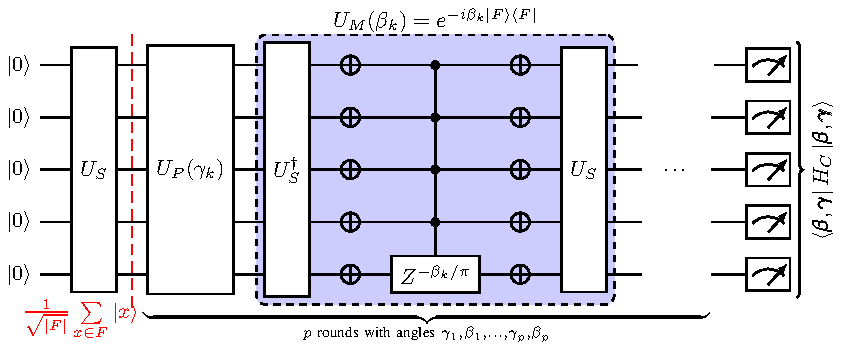
\includegraphics[width=0.6\textwidth]{figures/gm-qaoa}
    \caption[Circuit de l'ansatz quantique à opérateurs alternants avec forçage de Grover]{\textcolor{mydarkred}{\textit{Refaire la figure.}}}
    \label{fig:gm-qaoa}
\end{figure}

L'innovation principale de travail provient de l'opérateur de mélange $U_{D}$, défini comme:

\begin{equation}
    U_D^{\mathrm{Grover}} = e^{-i \beta \ket{F}\!\bra{}} = U_{S}\left[ \mathds{1}^{\otimes n} -\left(1-e^{-i \beta}\right) (\ket{0}\!\bra{0})^{\otimes n} \right] U_{S}^{\dagger} \,.
\end{equation}

Cet opérateur ressemble aux opérateurs de diffusion utilisés dans l'algorithme d'amplification d'amplitude, où les opérateurs de déphasage $e^{-i\beta}$ remplacent les opérateurs d'inversion de phase $e^{-i\beta}$. $U_{D}$ est alors implémenté en utilisant les unitaires $U_{S}$ et $U_{S}^{\dagger}$, deux couches d'opérateur de Pauli $X$ et un opérateur de déphasage $Z^{-\beta/\pi}$ contrôlés sur tous les qubits.

Une des conséquences de l'inspiration de l'algorithme de Grover signifie GM-QAOA peut préparer des superpositions égales d'états de même énergie. De plus, comme cette approche ne possède pas d'erreur de simulation d'Hamiltonien, comme les erreurs de Trotter. Notons que les problèmes NAE3SAT et 1-in-3SAT ne sont pas contraints et donc que l'espace faisable demeure le même que pour QAOA, c'est-à-dire que $\ket{F} = \ket{+}^{\otimes n}$.

%-----------------------------------------------------------------------------%

\section{Configuration des paramètres}
\label{subsec:configuration-des-parametres}

\begin{comment}
\subsection*{Plan}

\begin{enumerate}
    \item Décrire l'importance d'une bonne initialisation des paramètres (\textit{barren plateau}, non-convexité des paramètres)
    \item Énumérer les principales méthodes
    \item Expliquer l'initialisation aléatoire par grille
    \item Expliquer \textit{TQA}
\end{enumerate}

\subsection*{Références}

1. Bittel, L. and Kliesch, M. Training Variational Quantum Algorithms Is NP-Hard. Phys. Rev. Lett. 127, 120502 (2021).

2. Anschuetz, E. R. and Kiani, B. T. Beyond Barren Plateaus: Quantum Variational Algorithms Are Swamped With Traps. Nat Commun 13, 7760 (2022).

3. Akshay, V., Philathong, H., Morales, M. E. S. and Biamonte, J. D. Reachability Deficits in Quantum Approximate Optimization. Phys. Rev. Lett. 124, 090504 (2020).
    
4. Cain, M., Farhi, E., Gutmann, S., Ranard, D. and Tang, E. The QAOA gets stuck starting from a good classical string. Preprint at https://doi.org/10.48550/arXiv.2207.05089 (2022).

Peut-être une référence de plus qui traite directement des barrens plateau?
\end{comment}

La capacité d'entraînement des réseaux de neurones à partir d'une simple descente de gradient fut en partie à l'origine de leur succès retentissant sur de nombreux différents problèmes. L'optimisation des paramètres se fait simplement, même avec des fonctions de coût non convexe, tout en offrant de puissants résultats. Une des attentes des VQA fut de posséder ce même comportement et de pouvoir ainsi pousser les limites des algorithmes variationnels. En effet, l'optimisation classique des paramètres de QAOA fait partie intégrante du concept d'algorithme variationnel quantique. Grâce à celle-ci, il est en théorie possible de prendre avantage des algorithmes quantiques en recourant à des ordinateurs quantiques bruités. Cependant, de nombreuses embûches rendent présentement cette tâche difficile. 

D'abord, l'estimation du gradient de coût est difficile dans de nombreuses situations en raison de la présence de plateaux stériles~\cite{mccleanBarrenPlateausQuantum2018, laroccaReviewBarrenPlateaus2024}, où le gradient devient exponentiellement petit avec la taille du système. Un nombre exponentiel de mesures devient alors nécessaires pour pouvoir identifier la direction minimisant la fonction de coût. Ces complications se présentent surtout pour des circuits de grande profondeur, mais d'autres surgissent même pour ceux de petites tailles. Un grand nombre de minima locaux sont effectivement considérés comme pauvres, c'est-à-dire qu'ils possèdent une énergie petite par rapport au minimum global, augmentant la difficulté d'atteindre une solution approximative de bonne qualité~\cite{anschuetzQuantumVariationalAlgorithms2022}. De plus, l'optimisation des paramètres des VQA est \textsf{NP}-difficile, et donc intraitables dans le pire des cas~\cite{bittelTrainingVariationalQuantum2021}. Ces difficultés sont d'autant plus importantes comme la complexité de l'espace des paramètres augmente avec le nombre de paramètres d'un circuit, impliquant une plus grande difficulté d'optimisation pour les circuits profonds. 

Cet ensemble de complication implique alors qu'une bonne initialisation des paramètres est nécessaire au succès de QAOA. Des paramètres initiaux suffisamment près de l'extremum global peuvent contourner les problèmes énoncés précédemment. L'initialisation de bons paramètres demeure une question ouverte, mais plusieurs approches permettent d'amoindrir ces problèmes. Sack et Serbyn propose entre autres une stratégie d'initialisation basée sur le recuit quantique trottérisé (« Trotterized Quantum Annealing ») (TQA)~\cite{sackQuantumAnnealingInitialization2021}. Cette méthode, utilisée pour les simulations de ce travail, offre la même performance qu'un nombre exponentiel d'initialisations aléatoires. Comme vu à la section~\ref{subsec:discretisation-qaoa}, un juste milieu doit être choisi entre le temps d'évolution et les erreurs de Trotter. L'initialisation TQA trouve ainsi le temps d'évolution optimale à une profondeur de circuit $p$ fixe. Pour ce faire, la décomposition décrite à la section~\ref{subsec:discretisation-qaoa} est appliquée sur une grille uniformément discrétisée des temps d'évolution $t_{k} = k \Delta t$, avec $k = 1,\dots, p$, avec un pas de temps $\Delta t = T / p$. Les angles du circuit QAOA correspondant sont alors:

\begin{equation}
    \gamma_{i} = \frac{i}{p} \Delta t \,, \beta = (1 - \frac{i}{p}) \Delta t \,.
\end{equation}

Le pas de temps est optimisé de manière à minimiser la valeur moyenne de l'Hamiltonien de problème $H_{P}$, donnant des bons paramètres initiaux.

%-----------------------------------------------------------------------------%

\section{Échantillonnage et biais}
\label{sec:echantillonnage-et-biais}

\begin{comment} 
\subsection*{Plan}

\begin{enumerate}
    \item Expliquer l'importance de l'échantillonnage non-biaisé
    \item Expliquer le problème d'échantillonage associé au recuit quantique
    \item Expliquer le problème d'échantillonage associé à QAOA
    \item Expliquer pourquoi GM-QAOA résout ce problème (ne pas oublier d'expliquer les inconvénients de cette méthode)
\end{enumerate}

\subsection*{Références}

1. Zhang, Z. et al. Grover-QAOA for 3-SAT: Quadratic Speedup, Fair-Sampling, and Parameter Clustering. Preprint at https://doi.org/10.48550/arXiv.2402.02585 (2024).

2. Mandrà, S., Zhu, Z. and Katzgraber, H. G. Exponentially Biased Ground-State Sampling of Quantum Annealing Machines with Transverse-Field Driving Hamiltonians. Phys. Rev. Lett. 118, 070502 (2017).

3. Matsuda, Y., Nishimori, H. and Katzgraber, H. G. Ground-state statistics from annealing algorithms: quantum versus classical approaches. New J. Phys. 11, 073021 (2009).

Plus de sources sur le fair sampling pour QAOA?
\end{comment}

L'allure de la distribution obtenue par QAOA est dans notre cas essentiel. Afin de se conformer à la condition de l'algorithme de JVV, celle-ci doit être quasi uniforme comme sans ce critère l'algorithme de JVV n'offre aucune assurance.

Le recuit quantique n'échantillonne pas les états fondamentaux uniformément en général~\cite{matsudaGroundstateStatisticsAnnealing2009, mandraExponentiallyBiasedGroundState2017}. Certains états sont exponentiellement supprimés et nécessitent alors un nombre exponentiel de mesures pour être détectés. Comme le recuit quantique et QAOA sont fortement liés, il est ainsi peu probable que QAOA puisse échantillonner les états fondamentaux de manière uniforme.

Une propriété de l'algorithme GM-QAOA devient alors d'un intérêt considérable: l'équiprobabilité des états de même énergie. Les solutions sont encodées dans l'état fondamental de l'hamiltonien de problème, ceux-ci posséderont alors la même amplitude et donc la même probabilité. Ainsi, en ne considérant que les solutions, l'état préparé par le circuit GM-QAOA possède toujours une non-uniformité nulle. 


\begin{comment}
\end{comment}

\chapter{Comptage variationnel quantique}

%-----------------------------------------------------------------------------%

\subsection*{Plan}

\begin{enumerate}
    \item Expliquer que cette section ne concerne que GM-QAOA
\end{enumerate}

%-----------------------------------------------------------------------------%

\section{Auto-réductibilité des algorithmes variationnels quantiques}

\subsection*{Plan}

\begin{enumerate}
    \item Faire la preuve de l'auto-réductibilité des algorithmes variationnels quantiques
\end{enumerate}

\subsection*{Références}

%-----------------------------------------------------------------------------%

\section{Algorithme VQCount}

\subsection*{Plan}

\begin{enumerate}
    \item Vulgariser l'algorithme de manière général
    \item Expliquer rigoureusement l'algorithme
    \item Faire le lien entre la notation utilisée dans les algorithmes de comptage classique
    \item Faire la comparaison avec les travaux précédents
    \item Rajouter l'algorithme complet en pseudo-code
\end{enumerate}

\subsection*{Références}

% \begin{figure}[t]
%     \centering
%     \begin{quantikz}[font=\sffamily]
%       \ket{0} & \gate[style={fill=mysilver!80}][0.80cm]{H} & \gate[wires=4, nwires=3, style={fill=myblue}][1.30cm]{U_P (\alpha_{1})} & \gate[wires=4, nwires=3, style={fill=myred}][1.30cm]{U_D (\beta_{1})} & \ \ldots\ \qw & \gate[wires=4, nwires=3, style={fill=myblue}][1.30cm]{U_P (\alpha_{p})} & \gate[wires=4, nwires=3, style={fill=myred}][1.30cm]{U_D (\beta_{p})} & \qw \\
%       \ket{0} & \gate[style={fill=mysilver!80}][0.80cm]{H} & & & \ \ldots\ \qw & & & \qw \\
%       \vdots & & & & & & & \\
%       \ket{0} & \gate[style={fill=mysilver!80}][0.80cm]{H} & & & \ \ldots\ \qw & & & \qw
%     \end{quantikz}
%     \caption{}
% \end{figure}

% \begin{figure}[t]
%     \centering
%     \begin{quantikz}
%       \ket{0} & \gate[style={fill=myyellow!80}][0.80cm]{X^{c}} & \gate[wires=4, nwires=3, style={fill=myblue}][1.30cm]{U_P (\alpha_{1})} & \qw & \ \ldots\ \qw & \gate[wires=4, nwires=3, style={fill=myblue}][1.30cm]{U_P (\alpha_{p}) } & \qw & \qw \\
%       \ket{0} & \gate[style={fill=mysilver!80}][0.80cm]{H} & & \gate[wires=3, nwires=2, style={fill=myred}][1.30cm]{U_D (\beta_{1})} & \ \ldots\ \qw & & \gate[wires=3, nwires=2, style={fill=myred}][1.30cm]{U_D (\beta_{p})} & \qw \\
%       \vdots & & & & & & & \\
%       \ket{0} & \gate[style={fill=mysilver!80}][0.80cm]{H} & & & \ \ldots\ \qw & & & \qw
%     \end{quantikz}
%     \caption{}
% \end{figure}

\begin{figure*}[t]
    \centering
    \begin{subfigure}[h]{0.45\textwidth}
    \centering
    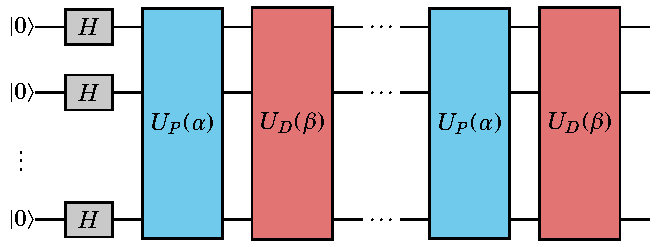
\includegraphics[width=1\textwidth]{figures/qaoa-self-reducibility-1.pdf}
    \caption{}
    \label{fig:quantum-circuit-a}
    \end{subfigure}
    \begin{subfigure}[h]{0.45\textwidth}
    \centering
    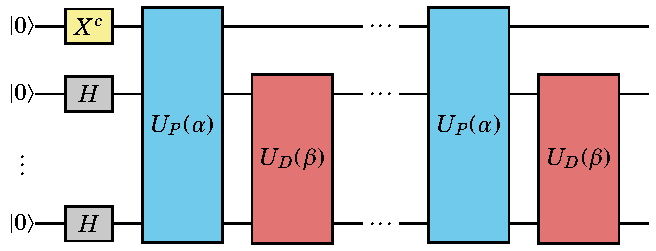
\includegraphics[width=1\textwidth]{figures/qaoa-self-reducibility-2.pdf}
    \caption{}
    \label{fig:quantum-circuit-b}
    \end{subfigure}
\caption{}
\label{fig:quantum-circuit}
\end{figure*}

%-----------------------------------------------------------------------------%

\section{Module VQCount}

\subsection*{Plan}

\begin{enumerate}
    \item Expliquer les librairies python dévelopées
    \item Décrire \textit{qaoa-quimb}
    \item Décrire \textit{VQCount}
\end{enumerate}

\subsection*{Références}

\begin{comment}
- Gibs phenomenon
- Post-processing used (how impactful is removing non-distinct solutions?)
- How does clean TVD evolve with JVV steps (see proof)?
- Approximation ratio
- Numerical analysis (which mean to take)
\end{comment}

    \chapter{Résolution de problèmes \textsf{\#P}-difficile}

%-----------------------------------------------------------------------------%

\subsection*{Plan}

\begin{enumerate}
    \item Mentionner les problèmes étudiés
    \item Mentionner les méthodes utilisées (réseaux de tenseurs)
    \item Décrire les paramètres de l'étude (nombre d'instances, régimes de complexité, etc.)
    \item Expliquer les principaux résultats (compromis entre QAOA et GM-QAOA)
\end{enumerate}

\subsection*{Références}

%-----------------------------------------------------------------------------%

\section{Biais d'échantillonage des problèmes \textsf{\#P}-difficile}

\subsection*{Plan}

\begin{enumerate}
    \item Décrire le comportement de la non-uniformité pour les différents problèmes (ne pas oublier 2SAT)
\end{enumerate}

\subsection*{Références}

%-----------------------------------------------------------------------------%


\section{Performance et comportement de l'algorithme VQCount}

\subsection*{Plan}

\begin{enumerate}
    \item  Décrire le taux de réussite et le nombre d'échantillons requis
    \item  Décrire la performance de l'algorithme en fonction de la profondeur du circuit
    \item Décrire l'efficacité d'échantillonage et la précision du compte
    \item Présenter brièvement le ratio d'approximation
\end{enumerate}

\subsection*{Références}

%-----------------------------------------------------------------------------%

\section{Transitions de phase observées par l'algorithme VQCount}

\subsection*{Plan}

\begin{enumerate}
    \item 
\end{enumerate}

\subsection*{Références}

%-----------------------------------------------------------------------------%


\Conclusion % Chapitre qui ne sera pas numéroté si IntroConcluSansNombre est Vrai

%-----------------------------------------------------------------------------%

Ce travail introduit VQCount, un algorithme variationnel quantique basé sur l'algorithme de JVV pour le comptage approximatif de modèles à partir de l'échantillonnage aléatoire de l'état préparé par QAOA. La validité de VQCount est établie dans une limite où la forme de l'algorithme de Grover est retrouvée. Comparativement à des travaux précédents, VQCount nécessite un nombre d'échantillons exponentiellement plus petit pour obtenir une estimation à un facteur multiplicatif près du compte exact lorsque le nombre de solutions est exponentiel. La performance de VQCount est étudiée numériquement en tant que méthode heuristique, en utilisant la contraction de réseaux de tenseurs pour simuler les circuits quantiques composant l'algorithme. Pour les problèmes de dénombrement \#NAE3SAT et \#1-in-3SAT, un compromis est établi entre le taux de succès et l'uniformité de l'échantillonnage de solutions. 


L'algorithme VQCount n'introduit que la fondation d'un algorithme variationnel quantique pour le comptage. La seule technique de post-traitement utilisée est le rejet des échantillons n'appartenant pas à l'ensemble de solutions, mais des techniques plus élaborées, comme la mise à jour de clusters sans rejet à température nulle~\cite{ochoaFeedingMultitudePolynomialtime2019}, pourrait être employée. Les algorithmes de comptage approximatif basés sur l'échantillonnage aléatoire ont aussi grandement évolués depuis le travail de Jerrum, Valiant et Vazirani. Par exemple, une modification de l'algorithme de JVV permet d'offrir des garanties sur le compte approximatif obtenu même pour des distributions de solutions non-uniforme~\cite{gomesSamplingModelCounting2007}.




%-----------------------------------------------------------------------------%

\singlespacing

\appendix
\renewcommand\chapterstring{Annexe}

\begin{comment}
\end{comment}

\appendix
\renewcommand\chapterstring{Annexe}

\chapter{Expression fermée de l'état du circuit GM-QAOA}
\label{ann:expression-fermee-etat-circuit-gm-qaoa}

%-----------------------------------------------------------------------------%

\begin{maintheorem}{Expression fermée de l'état du circuit GM-QAOA}{expression-fermee-etat-gm-qaoa}
    Pour un espace de solutions non contraint, l'état préparé par un circuit GM-QAOA $\ket{\psi(\vec{\gamma}, \vec{\beta})}$ de profondeur $p$ pour $n$ qubits s'exprime sous la forme de l'expression récursive fermée suivante:
    \begin{equation}
        \label{eq:recursive-formula}
        \ket{\psi} = \frac{1}{\sqrt{ N }} \left( \sqrt{ \lvert G \rvert } F_{p} \ket{g} + \sum_{k} \sqrt{ \lvert E^{(k)} \rvert } \bar{F}^{(k)}_{p} \ket{e^{(k)}} \right) \,,
    \end{equation}
    où $N=2^{n}$, $F_{0}=\bar{F}_{0}^{(k)}=1$ et
    \begin{align}
        F_{p} &= F_{p-1} - \frac{1}{N} (1-e^{-i\beta_{p}}) \left( \lvert G \rvert   F_{p-1} + \sum_{k'} \lvert E^{(k')} \rvert \bar{F}^{(k')}_{p-1} e^{-i\gamma_{p}\varepsilon_{k'}} \right) \,, \\
        \bar{F}^{(k)}_{p} &= e^{-i\gamma_{p} \varepsilon_{k}}\bar{F}_{p-1}^{(k)} - \frac{1}{N} (1-e^{-i\beta_{p}}) \left( \lvert G \rvert   F_{p-1} + \sum_{k'} \lvert E^{(k')} \rvert \bar{F}^{(k')}_{p-1} e^{-i\gamma_{p}\varepsilon_{k'}} \right) \,,
    \end{align}
    pour les états fondamentaux $\ket{g} \in G$ et les états excités $\ket{e^{(k)}} \in E^{(k)}$ de niveau $k$.
\end{maintheorem}

\begin{proof}
    
Soit $\varphi$ l'instance d'un problème de \textsf{\#P} de taille $n$ que nous voulons résoudre avec GM-QAOA. Cette instance peut être encodée dans un hamiltonien de problème $H_{P}$ avec des valeurs propres $g = 0$ pour les solutions et $e^{(k)} = \varepsilon_{k} \in \mathbb{R}_{>0}$ pour les non-solutions. L'opérateur $U_{P}$ correspondant avec $H_{P}$ s'écrit alors comme
\begin{equation}
    U_{P} = \sum_{j \in G} \ket{j}\bra{j} + \sum_{k} e^{-i \gamma \varepsilon_{k}} \sum_{j \in E^{(k)}} \ket{j}\bra{j} \,,
\end{equation} 
où $G$ et $E^{(k)}$ sont respectivement les variétés des états fondamentaux et états excités, et donc l'ensemble des solutions et des non-solutions de $\varphi$. Pour un espace de solutions non contraint, l'opérateur $U_{D}^{GM}$ est donné par
\begin{equation}
    U_{D}^{GM} = \mathds{1} - (1 - e^{-i\beta}) (\ket{+}\!\bra{+}^{\otimes n}) \,.
\end{equation}
Les états fondamentaux et excités s'écrivent comme
\begin{align}
    \ket{g} = \frac{1}{\sqrt{ \lvert G \rvert }} \sum_{j \in G} \ket{j}, \\
    \ket{e^{(k)}} = \frac{1}{\sqrt{ \lvert E^{(k)} \rvert }} \sum_{j \in E^{(k)}} \ket{j} \,.
\end{align}
Montrons par induction que l'état final suit la formule récursive~\ref{eq:recursive-formula} en évoluant l'état initial $\ket{\psi_{0}} = \ket{+}^{\otimes n}$ avec un circuit GM-QAOA de $p$ couches. 

\paragraph{Cas 1 (1 couche):} Calculons $\ket{\psi_{1}} = U_{P}(\gamma_{1}) \ket{\psi_{0}}$.
\begin{equation}
\begin{aligned}
    \ket{\psi_{1}} & = \left(\sum_{j \in G} \ket{j}\bra{j} + \sum_{k} e^{-i \gamma_{1} \varepsilon_{k}} \sum_{j \in E^{(k)}} \ket{j}\bra{j} \right) \left( \frac{1}{ \sqrt{ N }} \sum_{j'=0}^{N-1} \ket{j'} \right) \\
    & = \frac{1}{ \sqrt{ N }} \left( \sum_{j \in G} \ket{j} + \sum_{k} e^{-i \gamma_{1} \varepsilon_{k}} \sum_{j \in E^{(k)}} \ket{j} \right) \\
    & = \frac{1}{ \sqrt{ N }} \left( \sqrt{ \lvert G \rvert  } \ket{g} + \sum_{k} \sqrt{ \lvert E^{(k)} \rvert  } e^{-i \gamma_{1} \varepsilon_{k}} \ket{e^{(k)}} \right) \,,
\end{aligned}
\end{equation}
où la relation $\sum_{j \in G}\ket{j}\bra{j} \sum_{j'=0}^{N} \ket{j'} = \sum_{j \in G} \ket{j}$ a été utilisée.

\noindent
Calculons désormais $\ket{\psi_{2}} = U_{D} (\beta_{1})\ket{\psi_{1}}$.
\begin{equation}
\begin{aligned}
    \ket{\psi_{2}} &= \left( \mathbb{1} - \frac{1}{N} (1 - e^{-i\beta_{1}}) \sum_{i',j'=0}^{N} \ket{i'}\!\bra{j'} \right) \left( \frac{1}{ \sqrt{ N }} \left( \sqrt{ \lvert G \rvert  } \ket{g} + \sum_{k} \sqrt{ \lvert E^{(k)} \rvert  } e^{-i \gamma_{1} \varepsilon_{k}}  \ket{e^{(k)}} \right) \right) \\
    &=  \frac{1}{ \sqrt{ N }} \left( \sqrt{ \lvert G \rvert  } \ket{g} + \sum_{k} \sqrt{ \lvert E^{(k)} \rvert  } e^{-i \gamma_{1} \varepsilon_{k}}  \ket{e^{(k)}} \right. \\
    &\left. - \frac{1}{N} (1 - e^{-i\beta_{1}}) \left( \lvert G \rvert + \sum_{k} \lvert E^{(k)} \rvert e^{-i \gamma_{1} \varepsilon_{k}} \right) \sum_{i'=0}^{N} \ket{i'} \right) \\
    &=  \frac{1}{ \sqrt{ N }} \left( \sqrt{ \lvert G \rvert  } \ket{g} + \sum_{k} \sqrt{ \lvert E^{(k)} \rvert  } e^{-i \gamma_{1} \varepsilon_{k}}  \ket{e^{(k)}} \right. \\
    & \left. - \frac{1}{N} (1 - e^{-i\beta_{1}}) \left( \lvert G \rvert + \sum_{k} \lvert E^{(k)} \rvert e^{-i \gamma_{1} \varepsilon_{k}}   \right) \left( \sqrt{ \lvert G \rvert  } \ket{g} + \sum_{k} \sqrt{ \lvert E^{(k)} \rvert } \ket{e^{(k)}} \right) \right) \\
    &= \frac{1}{\sqrt{ N }} \left( \sqrt{ \lvert G \rvert } F_{1} \ket{g} + \sum_{k} \sqrt{ \lvert E^{(k)} \rvert } \bar{F}^{(k)} \ket{e^{(k)}} \right)
\end{aligned}
\end{equation}
où 
\begin{align}
    F_{1} &= 1 - \frac{1}{N} (1 - e^{-i\beta_{1}}) \left(  \lvert G \rvert + \sum_{k'} \lvert E^{(k')} \rvert e^{-i \gamma_{1} \varepsilon_{k'}} \right) \\
    \bar{F}^{(k)}_{1} &= e^{-i\gamma_{1} \varepsilon_{k}} - \frac{1}{N} (1 - e^{-i\beta_{1}}) \left(  \lvert G \rvert + \sum_{k'} \lvert E^{(k')} \rvert e^{-i \gamma_{1} \varepsilon_{k'}} \right)
\end{align}
Le cas initial a donc été prouvé.

\paragraph{Cas 2 ($p$ couche):} Supposons que $\ket{\psi} = U_{D}(\beta_{p}) U_{P}(\gamma_{p}) \dots U_{D}(\beta_{1})U_{P}(\gamma_{1})\ket{\psi_{0}}$ donne lieu à la relation suivante
\begin{equation}
\begin{aligned}
    \ket{\psi} &= \frac{1}{\sqrt{ N }} \left( \sqrt{ \lvert G \rvert } F_{p} \ket{g_{i}} + \sum_{k} \sqrt{ \lvert E^{(k)} \rvert } \bar{F}^{(k)}_{p} \ket{e^{(k)}} \right) \,,
\end{aligned}
\end{equation}
où
\begin{equation}
\begin{aligned}
    F_{p} &= F_{p-1} - \frac{1}{N} (1-e^{-i\beta_{p}}) \left( \lvert G \rvert   F_{p-1} + \sum_{k'} \lvert E^{(k')} \rvert \bar{F}^{(k')}_{p-1} e^{-i\gamma_{p}\varepsilon_{k'}} \right) \\
    \bar{F}^{(k)}_{p} &= e^{-i\gamma_{p} \varepsilon_{k}}\bar{F}_{p-1}^{(k)} - \frac{1}{N} (1-e^{-i\beta_{p}}) \left( \lvert G \rvert   F_{p-1} + \sum_{k'} \lvert E^{(k')} \rvert \bar{F}^{(k')}_{p-1} e^{-i\gamma_{p}\varepsilon_{k'}} \right) \,.
\end{aligned}
\end{equation}

\paragraph{Cas 3 ($p+1$ couche):} En utilisant la supposition précédente, appliquons $U_{P}$ en calculant $\ket{\psi_{1}} = U_{P} \ket{\psi_{0}}$.
\begin{equation}
\begin{aligned}
\ket{\psi_{1}} & = \left(\sum_{j \in G} \ket{j}\bra{j} + \sum_{k} e^{-i \gamma_{p+1} \varepsilon_{k}} \sum_{j \in E^{(k)}} \ket{j}\bra{j} \right) \left( \frac{1}{\sqrt{ N }} \left( \sqrt{ \lvert G \rvert } F_{p} \ket{g} + \sum_{k} \sqrt{ \lvert E^{(k)} \rvert } \bar{F}^{(k)}_{p} \ket{e^{(k)}} \right) \right) \\
& = \frac{1}{\sqrt{ N }} \left( \sum_{j \in G_{i}} \ket{j}\bra{j} + \sum_{i=0}^{Q-1} \sum_{k} e^{-i \gamma_{p+1} \varepsilon_{k}} \sum_{j \in E^{(k)}_{i}} \ket{j}\bra{j} \right) \left( F_{p} \sum_{j \in G} \ket{j} + \sum_{k} \bar{F}^{(k)}_{p} \sum_{j \in E^{(k)}}\ket{j} \right) \\
& = \frac{1}{\sqrt{ N }} \left( F_{p} \sum_{j \in G}\ket{j}  + \sum_{k} \bar{F}^{(k)}_{p} e^{-i \gamma_{p+1} \varepsilon_{k}} \sum_{j \in E^{(k)}} \ket{j} \right) \\
& = \frac{1}{\sqrt{ N }} \left( \sqrt{ \lvert G \rvert  } F_{p} \ket{g} + \sum_{k} \sqrt{ \lvert E^{(k)} \rvert  }\bar{F}^{(k)}_{p} e^{-i \gamma_{p+1} \varepsilon_{k}} \ket{e^{(k)}} \right) \\
\end{aligned}
\end{equation}
Appliquons ensuite $U_{D}$ en calculant $\ket{\psi_{2}}=U_{D}\ket{\psi_{1}}$.
\begin{equation}
\begin{aligned}
\ket{\psi_{2}} &= \left( \mathbb{1} - \frac{1}{N} (1 - e^{-i\beta_{p+1}}) \sum_{i',j'=0}^{N} \ket{i'}\!\bra{j'} \right) \\
&\left( \frac{1}{\sqrt{ N }} \left( \sqrt{ \lvert G \rvert  } F_{p} \ket{g} + \sum_{k} \sqrt{ \lvert E^{(k)} \rvert  }\bar{F}^{(k)}_{p} e^{-i \gamma_{p+1} \varepsilon_{k}} \ket{e^{(k)}} \right) \right) \\
&= \frac{1}{\sqrt{ N }} \left( \left( \sqrt{ \lvert G \rvert  } F_{p} \ket{g} + \sum_{k} \sqrt{ \lvert E^{(k)} \rvert  }\bar{F}^{(k)}_{p} e^{-i \gamma_{p+1} \varepsilon_{k}} \ket{e^{(k)}} \right) \right. \\
& \left. - \frac{1}{N} (1 - e^{-i\beta_{p+1}}) \left(  \lvert G \rvert F_{p} + \sum_{k} \lvert E^{(k)} \rvert \bar{F}^{(k)}_{p} e^{-i \gamma_{p+1} \varepsilon_{k}}\right) \sum_{i'=0}^{N} \ket{i'} \right) \\
&= \frac{1}{\sqrt{ N }} \left( \sqrt{ \lvert G \rvert  } F_{p+1} \ket{g_{i}} + \sum_{k} \sqrt{ \lvert E^{(k)} \rvert  } \bar{F}^{(k)}_{p+1} e^{-i \gamma_{p+1} \varepsilon_{k}} \ket{e^{(k)}_{i}} \right) \\
\end{aligned}
\end{equation}
où
\begin{equation}
\begin{aligned}
F_{p+1} &= F_{p} - \frac{1}{N} (1-e^{-i\beta_{p+1}}) \left( \lvert G \rvert   F_{p} + \sum_{k'} \lvert E^{(k')} \rvert \bar{F}^{(k')}_{p} e^{-i\gamma_{p+1}\varepsilon_{k'}} \right) \\
\bar{F}^{(k)}_{p+1} &= e^{-i\gamma_{p+1} \varepsilon_{k}}\bar{F}_{p}^{(k)} - \frac{1}{N} (1-e^{-i\beta_{p+1}}) \left( \lvert G \rvert   F_{p} + \sum_{k'} \lvert E^{(k')} \rvert \bar{F}^{(k')}_{p} e^{-i\gamma_{p+1}\varepsilon_{k'}} \right)
\end{aligned}
\end{equation}  
La formule récursive a donc été prouvée par induction.
\end{proof}

%-----------------------------------------------------------------------------%


\chapter{Simulation de circuits quantiques avec les réseaux de tenseurs}
\label{ann:simulation-circuits-quantiques-avec-reseaux-de-tenseurs}

La simulation classique d'états quantiques est tout sauf évidente. Ces états, appartenant à l'espace de Hilbert, sont décrit par des vecteurs d'état de taille exponentielle empêchant ainsi leur caractérisation même pour des systèmes de taille modeste. Cette difficulté, présente dans de nombreux domaines, tel l'apprentissage automatique, est connue sous le nom de la \textit{malédiction de la dimensionnalité}. Cependant, la représentation de certains états physiques intéressants contient parfois de l'information superflue ou une structure inhérente. Par exemple, un état quantique général de $n$ qubits nécessite théoriquement un vecteur d'état à $2^{n}$ bits, mais un état quantique non intriqué nécessite seulement $2n$ bits en raison de l'absence de corrélation. Cette idée a alors mené au développement des méthodes de réseaux de tenseurs pour l'étude de système quantique à plusieurs corps en matière condensée afin d'obtenir une représentation des états quantiques plus efficaces.

Les réseaux de tenseurs font partie des méthodes les plus puissantes pour la simulation de circuits quantiques. Comme ceux-ci sont utilisés pour les simulations numériques présentées au chapitre~\ref{cha:resolution-de-problemes-avec-vqcount}, une brève introduction à la matière est nécessaire. Cette annexe décrit seulement en surface les méthodes de réseaux de tenseurs. Pour comprendre les différentes méthodes plus en profondeur, de nombreux excellents tutoriels ont été écrits~\cite{bridgemanHandwavingInterpretiveDance2017,biamonteTensorNetworksNutshell2017,bakerMethodesCalculAvec2021}. La section~\ref{sec:reseaux-de-tenseurs} introduit les réseaux de tenseurs ainsi que les principales opérations possibles. Une représentation alternative de ceux-ci, les états en produit de matrices, est décrite à la section~\ref{sec:mps-mpo} alors que la correspondance entre la simulation de circuits quantiques et la contraction de réseaux de tenseurs est expliquée à la section~\ref{sec:simulation-de-circuits-quantiques}.

%-----------------------------------------------------------------------------%

\section{Réseaux de tenseurs}
\label{sec:reseaux-de-tenseurs}

Un \textit{tenseur} est un tableau multilinéaire de rang, c'est-à-dire un nombre de dimensions, arbitraire encodant une certaine quantité d'information. Un tenseur s'interprète aussi comme une fonction définie sur un domaine discret. Par exemple, un scalaire, un vecteur et une matrice correspondent respectivement à un tenseur de rang 0, 1 et 2. Les tenseurs généralisent en outre ces derniers objets en admettant des tenseurs de rang $m$. 

\begin{subdefinition}{Tenseur}{tenseur}
    Un tenseur $T[x_{1}, x_{2}, \dots, x_{m}]$ de rang $m$ avec dimensions $d_{1} \times d_{2} \times \dots \times d_{m}$ est un élément de l'ensemble $\mathbb{C}^{d_{1} \times d_{2} \times \dots \times d_{m}}$.
\end{subdefinition}

Pour simplifier la notation, un tenseur s'écrit plus succinctement par $T[\varepsilon]$ où $\varepsilon \subseteq \set{ x_{1}, x_{2}, \dots, x_{m} }$. L'attrait principal des tenseurs est leur représentation géométrique simple, qui permet de visualiser aisément leurs caractéristiques principales ainsi que de faciliter leur manipulation. Tout tenseur $T$ se représente par une forme géométrique, où chaque indice $x_{i}$ est représenté par une patte sortant de la forme telle qu'illustrée à la figure~\ref{fig:tensor}. Un réseau de tenseurs est une collection de tenseurs $\set{ T_{1}[\varepsilon_{1}], T_{2}[\varepsilon_{2}], \dots, T_{n}[\varepsilon_{n}] }$ partageant certains indices $x_{i}$. La notation en réseaux de tenseurs s'apparente beaucoup à la notation d'Einstein; les sommations sont donc souvent implicites. 

\begin{figure}[h]
    \centering
    \begin{subfigure}[h]{0.2\textwidth}
        \centering
        \caption{}
        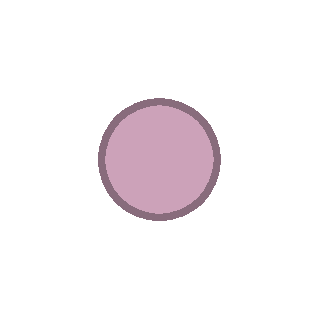
\includegraphics[width=1\textwidth]{figures/tensor-1.pdf}
        \label{fig:tensor-scalar}
    \end{subfigure}
    \begin{subfigure}[h]{0.2\textwidth}
        \centering
        \caption{}
        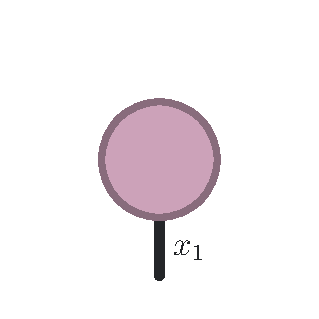
\includegraphics[width=1\textwidth]{figures/tensor-2.pdf}
        \label{fig:tensor-vector}
    \end{subfigure}
    \begin{subfigure}[h]{0.2\textwidth}
        \centering
        \caption{}
        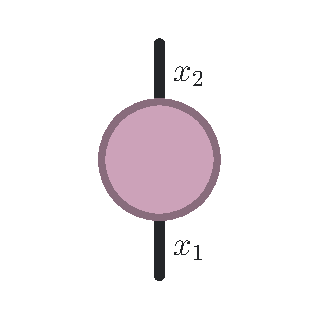
\includegraphics[width=1\textwidth]{figures/tensor-3.pdf}
        \label{fig:tensor-matrix}
    \end{subfigure}
    \begin{subfigure}[h]{0.2\textwidth}
        \centering
        \caption{}
        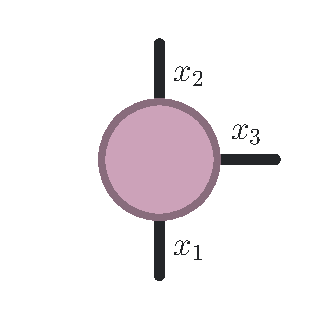
\includegraphics[width=1\textwidth]{figures/tensor-4.pdf}
        \label{fig:tensor-rank-3}
    \end{subfigure}
    \caption[Représentation géométrique des tenseurs]{Représentation géométrique de tenseurs de différents rangs. Des tenseurs de rang 0 (scalaire), 1 (vecteur), 2 (matrice) et 3 (tenseur de rang 3), sont illustrés respectivement aux panneaux (a), (b), (c) et (d).}
    \label{fig:tensor} 
\end{figure}

Plusieurs opérations peuvent être appliquées sur les tenseurs constituants d'un réseau de tenseurs. Le \textit{produit tensoriel} entre deux tenseurs $A$ et $B$ sur les ensembles d'indices respectifs $\varepsilon_{1}$ et $\varepsilon_{2}$ correspond au produit élément par élément des valeurs des tenseurs, généralisant ainsi le produit extérieur entre deux vecteurs

\begin{equation}
    (A \otimes B)[\varepsilon_{1}, \varepsilon_{2}] \coloneq A[\varepsilon_{1}] \cdot B[\varepsilon_{2}] \,.
\end{equation}

Le produit tensoriel se visualise simplement par la juxtaposition des deux tenseurs. La \textit{trace} (partielle) d'un tenseur $A$ est la sommation jointe sur deux indices $x_{i}$ et $x_{j}$ de $A$ ayant la même dimension $d_{x_{i}} = d_{x_{j}}$

\begin{equation}
    \text{Tr}_{x_{i}, x_{j}} (A[x_{i}, x_{j}, \varepsilon \setminus \set{x_{i}, x_{j}}]) \coloneq \sum_{k}^{d_{x_{i}}} A[k, k, \varepsilon \setminus \set{x_{i}, x_{j}} ] \,. 
\end{equation}

Géométriquement, la trace implique de joindre les pattes du tenseur. La \textit{contraction} de deux tenseurs est l'opération la plus commune, consistant en un produit tensoriel entre deux tenseurs $A$ et $B$ suivi d'une trace entre les indices communs $\partial \varepsilon$ de ces derniers

\begin{equation}
    C[\varepsilon \setminus \set{ \partial \varepsilon}] \coloneq  \sum_{\partial \varepsilon} (A \otimes B)[\partial \varepsilon,  \varepsilon \setminus \set{ \partial \varepsilon}]
\end{equation}

Deux tenseurs contractés se combinent alors en une seule forme géométrique avec des pattes correspondant aux indices non contractés. Comme les tenseurs ne sont en réalité que des tableaux multidimensionnels, il est possible de réorganiser l'information encodée sous une différente forme. Les opérations de \textit{regroupement} et de \textit{séparation} modifient l'organisation de cette information. Par exemple, une matrice représentée par une matrice de taille $d_{1} \times d_{2}$ peut aussi être encodée dans un vecteur de taille $d_{1} \cdot d_{2}$. Cette manipulation des données se représente graphiquement par un regroupement ou une séparation des pattes des tenseurs.

Finalement, l'opération inverse à la contraction est la \textit{décomposition}, où un tenseur est décomposé en deux différents tenseurs. Un exemple particulièrement intéressant est la \textit{décomposition en valeurs singulières}, une méthode typiquement appliquée aux matrices, mais pouvant se généraliser aux tenseurs en les regroupant sous forme de matrices. Cette décomposition permet de plus de réduire la dimension des indices et donc de retirer l'information superflue en retirant les valeurs négligeables de la matrice singulière.

Les méthodes de réseaux de tenseurs suivent couramment la démarche suivante. Le problème à résoudre est d'abord modélisé sous la forme d'un réseau de tenseurs en encodant les contraintes sous la forme de tenseurs, de façon à ce que la contraction de ce réseau donne la solution au problème. En utilisant les opérations précédentes, incluant potentiellement les opérations de décomposition pour la simplification, le réseau est contracté pour obtenir la solution souhaitée. Notons que l'ordre de contraction, c'est-à-dire l'ordre dans lequel chacun des tenseurs est contracté avec les tenseurs environnants, à un fort impact sur la quantité de ressources nécessaires~\cite{grayHyperoptimizedTensorNetwork2021}.

%-----------------------------------------------------------------------------%

\section{État en produit de matrices et opérateur en produit de matrices}
\label{sec:mps-mpo}

Un \textit{état en produit de matrices} (« Matrix Product State ») (MPS) est un type particulier de réseau de tenseurs permettant la représentation efficace d'un état quantique. Considérons un état quantique $\ket{\psi}$ à $n$ qubits. En employant la notation en réseau de tenseurs, cet état se représente par un tenseur de rang $n$, avec $n$ indices de dimensions $d=2$, encodant les amplitudes des qubits de $\ket{\psi}$. Cette représentation nécessite un grand nombre d'éléments, plus précisément $2^{n}$, pour encoder l'entièreté des amplitudes des qubits. Alternativement, ce tenseur peut être décomposé en $n$ tenseurs à l'aide de la décomposition en valeurs singulières. Ce nouveau réseau de tenseurs, illustré à la figure~\ref{fig:mps}, représente alors un MPS. En coupant les plus petites valeurs de la matrice singulière lors de la décomposition, correspondant à l'information redondante du système, une représentation de taille réduite peut être obtenue, permettant ainsi l'étude de l'état souhaité. Les MPS sont particulièrement utiles pour l'étude de l'intrication entre deux sous-parties d'un système comme celle-ci est capturée dans les indices latéraux du MPS. Notons que la taille de la représentation sous forme de MPS est grandement dépendante de l'intrication du système. Un système fortement intriqué ne possède pas de représentation efficace à l'aide de ce type d'objet.

\begin{figure}[h]
    \centering
    \begin{subfigure}[h]{0.7\textwidth}
        \centering
        \caption{}
        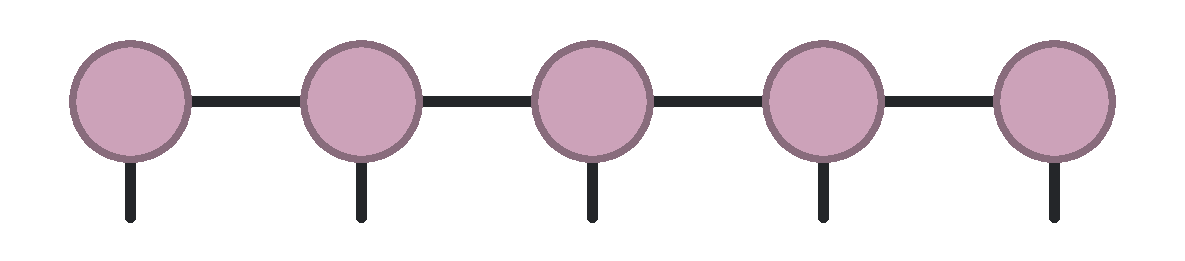
\includegraphics[width=1\textwidth]{figures/mps.pdf}
        \label{fig:mps}
    \end{subfigure}
    \begin{subfigure}[h]{0.7\textwidth}
        \centering
        \caption{}
        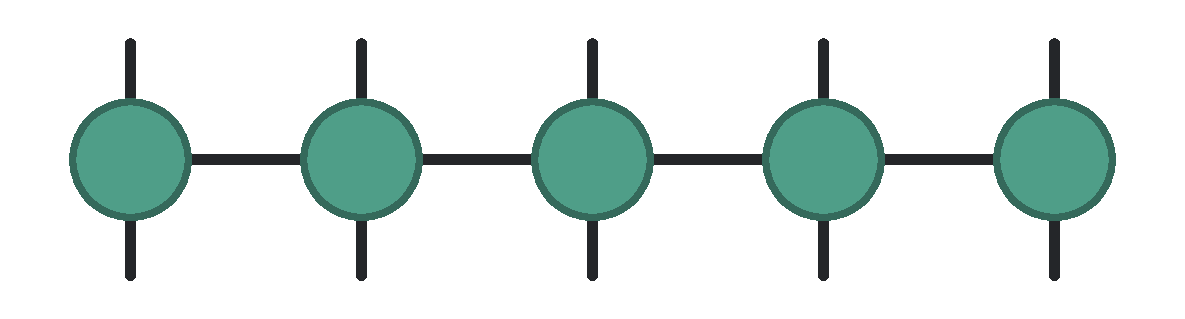
\includegraphics[width=1\textwidth]{figures/mpo.pdf}
        \label{fig:mpo}
    \end{subfigure}
    \caption[État et opérateur en produit de matrices]{Schéma d'un état (a) et d'un opérateur (b) en produit de matrices.}
\end{figure}

Les opérateurs en produit de matrices permettent quant à eux d'appliquer un opérateur sur un MPS. Ces opérateurs empruntent la forme d'un MPS en rajoutant une patte par tenseur tel qu'illustré à la figure~\ref{fig:mpo}. La méthode MPS/MPO peut par exemple représenter l'évolution d'un système quantique selon un certain hamiltonien (représenté sous forme de MPO). Ces opérateurs permettent de plus de représenter les matrices de densités. Encore une fois, l'utilité de ceux-ci dépend grandement de l'intrication qu'ils ajoutent au MPS.

%-----------------------------------------------------------------------------%

\section{Simulation de circuits quantiques}
\label{sec:simulation-de-circuits-quantiques}

Les réseaux de tenseurs font partie des méthodes les plus performantes pour la simulation de circuits quantiques. Il y a en effet une correspondance parfaite entre les réseaux de tenseurs et les circuits quantiques. L'état d'un qubit s'encode facilement par un tenseur de rang $d = 1$. Par exemple, pour un qubit dans une superposition égale, l'état est représenté par le tenseur
\begin{equation}
    T^{\ket{\psi}} = \frac{1}{\sqrt{2}}
    \begin{pmatrix}
        1 \\
        1
    \end{pmatrix} \,.
\end{equation}
De plus, les opérateurs d'un circuit quantique se représentent aussi simplement par des tenseurs. Par exemple, une porte de Pauli $X$ correspond à un tenseur 
\begin{equation}
    T^{X} = 
    \begin{pmatrix}
        0 & 1 \\
        1 & 0
    \end{pmatrix}
\end{equation}
de rang $d = 2$. La contraction d'un réseau composé des différents opérateurs d'un circuit donné est alors équivalente à l'état obtenu par l'application d'opérateurs quantiques. La méthode MPS/MPO se prête bien à la simulation de circuit quantique, particulièrement lorsque l'intrication de celui-ci demeure faible. Les simulations effectuées au cours du travail de ce mémoire emploient alors autant la contraction de réseaux de tenseurs sans forme précise que la contraction de MPS/MPO, selon l'efficacité de la méthode pour un problème étudié.

Afin d'obtenir des échantillons à partir d'un réseau de tenseurs, deux méthodes sont possibles. D'abord, une représentation dense de la fonction d'onde peut être obtenue en contractant complètement le réseau. Les configurations sont alors simplement obtenues en pigeant selon la distribution de probabilité trouvée. Cette stratégie exige de sauvegarder un nombre exponentiel de valeurs, ce qui est infaisable pour des instances de grandes tailles. Une méthode alternative est plutôt la méthode proposée par Ferris et Vidal~\cite{ferrisPerfectSamplingUnitary2012}. Pour mesurer la valeur moyenne d'opérateurs locaux, les cônes causaux passés de ceux-ci sont utilisés pour éviter de contracter l'entièreté du réseau de tenseurs. Une séquence de matrices de densité conditionnelles est alors calculée en contractant un à un les opérateurs du cône causal pour permettre l'échantillonnage de la distribution de probabilités des configurations. Cette approche garantit un échantillonnage parfait, c'est-à-dire qu'il est possible d'obtenir des échantillons totalement non corrélés directement de la distribution de probabilités exacte. L'implémentation de cette méthode dans la librairie « quimb »~\cite{grayQuimbPythonPackage2018} est utilisée dans ce mémoire pour réduire la complexité de l'échantillonnage.

%-----------------------------------------------------------------------------%


%=============================================================================%

% Voir switchboard.tex pour le bibliographystyle selon le type de document.
\printbibliography        % Le fichier de bibliographie est memoire.bib.

\end{document}
